%\documentclass[a4paper,uplatex]{jsarticle,jsotsuron}
\documentclass[12pt , twoside]{jsotsuron}
\usepackage{newtxtext}
\usepackage{textcomp}
\usepackage[sc]{mathpazo}
\usepackage{amsmath,amssymb,arydshln, amsthm}
\usepackage[scaled]{helvet}
\usepackage{otf}
\usepackage[dvipdfmx]{graphicx,xcolor}
\usepackage{tikz}
\usepackage[framemethod=tikz]{mdframed}
\usepackage{float}
\usepackage{subcaption}
\usepackage{verbatim}
\usepackage{ascmac}
%\usepackage{algorithm, algorithmic}
\usepackage{listings,jlisting}
\usepackage{bm}

\usepackage{algorithm, algpseudocode}

\usepackage{color}
\usepackage{pgfplots}
\usepackage{tikz}
\usepackage{longtable}
\usepackage{comment}
\usepackage{multirow}
\usepackage{url}

\usetikzlibrary{positioning}
\usetikzlibrary{arrows.meta}
\usetikzlibrary{quotes}
\usetikzlibrary{shapes}
\usetikzlibrary{backgrounds}
\usetikzlibrary{fit}

\lstset{%
	language={C},
	basicstyle={\small},%
	identifierstyle={\small},%
	commentstyle={\small\itshape},%
	keywordstyle={\small\bfseries},%
	ndkeywordstyle={\small},%
	stringstyle={\small\ttfamily},
	frame={tb},
	breaklines=true,
	columns=[l]{fullflexible},%
	numbers=left,%
	xrightmargin=0zw,%
	xleftmargin=3zw,%
	numberstyle={\scriptsize},%
	stepnumber=1,
	numbersep=1zw,%
	lineskip=-0.5ex%
}

\theoremstyle{definition}
\newtheorem{theorem}{定理}
\newtheorem*{theorem*}{定理}
\newtheorem{definition}[theorem]{定義}
\newtheorem*{definition*}{定義}
\newtheorem{lemma}[theorem]{補題}
\newtheorem*{lemma*}{補題}
\newtheorem{Proof}{証明}
\newtheorem*{Proof*}{証明}

\newcommand{\argmax}{\mathop{\rm arg~max}\limits}
\newcommand{\argmin}{\mathop{\rm arg~min}\limits}
% RequireとEnsureをInputとOutputにする
\renewcommand{\algorithmicrequire}{\textbf{Input:}}
\renewcommand{\algorithmicensure}{\textbf{Output:}}

\title{ 最大クリーク発見に関する省メモリアルゴリズム\\
 A Space Efficient Algorithm\\ for Finding A Maximum Clique}
\author{小畠 教寛\\ Norihiro Obata}

\date{令和2年2月}

\begin{document}
\maketitle
%$ $
%\newpage

\begin{abstract}
%アブストラクトを書く.
無向グラフから最大クリークを1つ発見する問題は,NP困難に属する組み合わせ最適化問題である.
現実の様々な問題が,最大クリーク抽出やそれに類する問題として,モデル化できることから,
最大クリーク問題は,工学的に重要な問題となっている.
%最大クリーク抽出の効率の良いアルゴリズムが提案されている.
最大クリーク抽出のアルゴリズムとして,彩色による分枝限定法を用いた高速なアルゴリズムが,
Tomitaらによって提案されている.
%
このアルゴリズムは,省メモリ化に対しては,多く研究されていない.
%最大クリークを発見するアルゴリズムは,高速化する研究は古くから研究されているが,省メモリ化についてはあまり研究をされていない.
%
本論文では,最大クリークが巨大なグラフに対しても実用上で,解を得られるように
最大クリークを発見する省メモリで動作するアルゴリズムを提案する.
%最大クリーク抽出の省メモリアルゴリズムに対する提案をする.
実験において,提案アルゴリズムは,最大クリークのサイズが,
大きなグラフに対して,最大メモリ使用量が1MBから7MB程度に減少することが確認された.

\end{abstract}
\newpage
\tableofcontents
\newpage

%%%%%%%%論文本体%%%%%%%%
\chapter{はじめに}
\label{ch:intro}
\section{背景}
最大クリークを発見する問題は,NP困難問題のクラスに属する組合せ最適化問題の一つとして古くから研究されている問題である\cite{Karp1972}.
現実の様々な問題が,最大クリークの発見やそれに類する問題としてモデル化できることから,
最大クリークを発見する問題は,工学的に重要な問題となっている.

%応用例としては,経済学\cite{BOGINSKI20063171}や符号理論\cite{etzion1998greedy}などが挙げられる.
%最大クリークを抽出する高速なアルゴリズムは今なお研究されている.
たとえば,株式市場におけるマーケットグラフ(market graph)の最大クリークは重要な特徴を表す.
%マーケットグラフでの最大クリークは,株式市場での重要な特徴を表す.
%マーケットグラフは次のように構成される.
%頂点を株とし,2つの頂点が辺で接続されていることと2つの株価の相関係数が閾値を超えていることが一致している.
マーケットグラフとは,各株の銘柄を頂点とし,
株価の相関係数がある閾値を超える頂点どうしを辺で接続したグラフである.
閾値を高い値にすると,辺が存在することは,2つの株に重要な相関関係があることを表す.
%このグラフのクリークのどの頂点も同じクリークに属する他の頂点に似た振る舞いをしていることを表す.
グラフのクリークに含まれる頂点に対応する株は,似た振る舞いをしていることを表す.
したがって,最大クリークは,株式市場における似た振る舞いをする株の最大のグループという特徴を表す\cite{BOGINSKI20063171}.
\section{関連研究}
\label{sec:relation}
%無向グラフから最大クリークを1つ抽出する問題に関して実働上で効率良く解を得ることを目的としたアルゴリズムが日々研究され開発されている.

グラフから最大クリークの厳密解を求めるアプローチのほとんどは,分枝限定法を基にしている.
%異なることは,
厳密解を求める各アルゴリズムの違いは,
主に上界と下界を決定する手法と分岐の戦略である.
1990年に,CarraghanとPardalos \cite{carraghan1990exact}は,
%多くの後の分枝限定法の基礎となるシンプルな
2つの工夫を用いた単純なアルゴリズムを提案している.
1つ目は,常に次数最小の頂点を選べるように頂点を整列させることである.
2つ目は,クリークに全ての頂点を加えても最大クリークを更新できなくなったら探索を打ち切ることである.
%頂点を常に次数最小の順に選べるように頂点を整列させてから,クリークに全ての頂点を加えても最大クリークを更新できなくなったら探索を打ち切るという単純な分枝条件の
%アルゴリズムを提案している.
これは,後の厳密解を求める多くのアルゴリズムに影響を与えた.
同年,BabelとTinhofer \cite{Babel1990}は,彩色を用いることで最大クリークの上界の決定することによって分枝限定をより効率的に探索するアルゴリズムを提案している.
その後,2003年にTomita \cite{tomita2003efficient}らは,彩色による分枝限定法によるアルゴリズムでMCQが提案している.
さらに,Tomitaらはそれを改善したアルゴリズムとして,2007年にMCR \cite{tomita2007efficient}を,
2010年にMCS \cite{tomita2010simple}\cite{tomita2013simple}を,2016年にMCT \cite{tomita2016much}を提案している.
%また,それを改善したアルゴリズムとしてMCR(2007)\cite{tomita2007efficient},MCS(2010)\cite{tomita2010simple}\cite{tomita2013simple},MCT(2016)\cite{tomita2016much}などの高速な最大クリーク抽出アルゴリズムが提案されている.

一方,グラフから最大クリークの近似解を高速に求める手法が提案されている.
この手法のアプローチには,貪欲な手法%\cite{DBLP:journals/jgo/PardalosX94a}や
と局所探索法がある.
貪欲な手法の1つとして,2004年にGrossoらは,
DAGS \cite{DBLP:journals/heuristics/GrossoLC04}を提案している.
これは,現在のクリークをより有望なクリークに変換することと頂点に重みをつけるという2点の工夫を用いたアルゴリズムである.
局所探索法の1つとして,2005年にKatayamaらは,
$k$-opt Local Search(KLS) \cite{katayama2005effective}を提案している.
これは,クリークに頂点を追加・削除することで生成可能な解の集合を
近傍と捉えて探索を行うアルゴリズムである.

\section{目的}
%\section{内容}
%Tomitaらの提案しているMCQと,MCR,MCS,MCTは省メモリ化についてあまり研究をされていない.
MCSは,深さ優先探索に基づく最大クリークを発見するアルゴリズムである.
MCSのメモリ使用量のボトルネックは,深さ優先探索の各段階は,各段階の探索が終了まで,頂点集合などの情報を
コピーして保持する必要があることである.
このため,最大クリークが大きいとき,探索が深くなりやすいので,メモリ使用量も大きくなる.

本論文では,最大クリークが巨大なグラフに対しても実用上で解を得られるように
%本論文では巨大なグラフに対してもアルゴリズムが適用できるように,
%アルゴリズムの
最大メモリ使用量の削減に着目をして取り組んだ.%目的
%本論文では,
我々は,TomitaらのMCSに基づく,その省メモリ化の手法を提案する.
省メモリ化のアイデアとしては,深さ優先探索で子に進む際に捨てる情報のみを保持し,
子には,頂点集合の情報をコピーせずに渡すことで省メモリ化を行う.
%バックトラックした後に,彩色アルゴリズムを再び適用することで,探索順序を決定する.
MCTでは,部分問題に応じて彩色アルゴリズムを切り替える.
彩色アルゴリズムの1つは親の彩色を引き継ぐため,その情報を保存する必要がある.
このため,省メモリ化のアイデアを適用できないので,
MCSを改善したMCTではなく,MCSを基にした.

提案アルゴリズムと基にしたMCSに比較して,空間計算量や時間計算量が,改善したかどうかを調べる.
私がみる限り,Tomitaらは,MCSアルゴリズムに対して,空間計算量
%や時間計算量
を記載していない.
したがって,MCSと提案アルゴリズムの両方に対して,空間計算量と時間計算量についての解析を行う.
さらに,提案手法を実装し,35個のグラフに対して実験を行う.
実験に使用したグラフは,DIMACSベンチマークセットのグラフ\footnote{\url{http://iridia.ulb.ac.be/~fmascia/maximum_clique/DIMACS-benchmark}}
とクリークサイズの大きなグラフから辺をいくつか削除することで作成したグラフ, 
DIMACSのグラフのいくつかのグラフを合体させて,そのグラフ間に辺をランダムに引くことによって作成したグラフ
の3種類を用意した.

\section{結果}
 $n$はグラフのサイズ,$m$は辺の本数,$\omega$を最大クリークのサイズとする.

本論文の主な貢献は,以下の5点である.
\begin{itemize}
    \item MCSアルゴリズムの隣接行列表現から隣接リスト表現へ適用した.
    \item MCSアルゴリズムを基にした省メモリなアルゴリズムを提案をした.
    \item MCSアルゴリズムと提案アルゴリズムの空間計算量について解析を行った.
	空間計算量について,まとめたものが,表\ref{tab:result-mem}である.
	提案アルゴリズムの隣接リスト表現の空間計算量$O(n+m)$が,MCSアルゴリズムの$O(n \omega + m )$に対して小さく抑えられることを示した.
    %\item MCSアルゴリズムと提案アルゴリズムの再帰処理の時間計算量についての解析を行った.
%	提案アルゴリズムの再帰処理の時間計算量が隣接行列で$O(n^4)$時間である.
%	これは,MCSアルゴリズムの$O(n^3)$時間に対して悪化している.
%	また,隣接リスト表現についても提案アルゴリズムは$O(n^4 \log n )$時間である.
%	これは,MCSアルゴリズムの$O(n^3 \log n )$時間に対して悪化している.
    \item %MCSアルゴリズムの再帰処理の時間計算量は,隣接行列表現で$O(n^3)$時間,隣接リスト表現で$O(n^3 \log n )$時間であることを示した.
	%さらに,
	提案アルゴリズムの再帰処理の時間計算量は,隣接行列表現で$O(n^4)$時間,隣接リスト表現で$O(n^4 \log n)$時間であることを示した.

    \item MCSアルゴリズムと提案アルゴリズムの2つのアルゴリズムに対して,35個のグラフでの実験を行った.
	最大クリークのサイズの大きい14個のグラフに対して,最大メモリ使用量の削減を確認し,その効果に対しての考察を行なった.
	%
実験に使用したグラフは,DIMACSベンチマークセットのグラフ\footnotemark[1]
とクリークサイズの大きなグラフから辺をいくつか削除することで作成したグラフ, 
DIMACSのグラフのいくつかのグラフを合体させて,そのグラフ間に辺をランダムに引くことによって作成したグラフ
の3種類を用意した.

\end{itemize}
 %$n,m,w$では,
%関連研究として,鳥谷部\cite{toriyabe}は○○を発見した.

\begin{table}[p]
\centering
\caption{アルゴリズムの空間計算量}
\label{tab:result-mem}
    \begin{tabular}{|l|l|l|}
\hline
 & MCSアルゴリズム &  提案アルゴリズム   \\ \hline
隣接行列 & $O(n^2)$ & $O(n^2)$  \\ \hline
隣接リスト & $O(n \omega +m )$ & $ O(n + m ) $   \\ \hline

\end{tabular}
    \begin{center}
    \small{  $n$はグラフのサイズ$|V|$,$m$はグラフの辺の数$|E|$,$\omega$はグラフの最大クリークのサイズ }
    \end{center}
\end{table}



\section{本論文の構成}
本論文の構成は,次の通りである.
%\begin{itemize}
%\item 
第2章では,グラフの基本的な定義やグラフの表現について記述する.
%\item 
第3章では,最大クリーク抽出アルゴリズムの基本的なアイデアについて説明する.
%\item 
第4章では,MCSアルゴリズムを基づく提案アルゴリズムについて説明し,その空間計算量や時間計算量について記述する.
%\item
第5章では,実験結果を記載して,結果に対して考察する.
%\item 
第6章では,本論文のまとめと今後の課題について述べる.
%\end{itemize}

\chapter{準備}
\label{ch:prelm}

本章では,
本論文で用いる基本的なグラフに関する定義と記法を導入する.
%後の章で必要となる基本的な概念と定義を導入する.
まず,\ref{sec:graph}節では,グラフの基本的な定義をする.
次に,\ref{sec:graph_represetion}節では,グラフの表現方法について説明する.
\section{グラフ}
\label{sec:graph}
この節では,グラフの諸定義を行う.
本論文では,$[A]^k := \{ X \subseteq A | |X| = k \}$とする.
%本論文では,$[A]^2 := \{ X \subseteq A | |X| = 2 \}$とする.
%は,$A$の冪集合の中で,2要素からなる全て集合を要素とした集合とする.
%本論文では,$[A]^2$は,$A$の冪集合の中で,2要素からなる全て集合を要素とした集合とする.
ここで,$V$を有限集合,$E \subseteq [V]^2$とする.

\subsection*{無向グラフ}
無向グラフは,対$G=(V,E)$である.
この集合$V$を$G$の頂点集合と呼び,集合$E$を$G$の辺集合と呼ぶ.
$V$の各要素は,頂点と呼ぶ.
$E$の各要素は,辺と呼ぶ.%辺は$V$の2つの要素の部分集合である.
%辺は,$V$の部分集合でサイズが2のものである.

無向グラフの例として,
\begin{eqnarray*}
    V &=& \{ 1,2,3,4,5,6 \} \\
    E &=& \{ \{1,2\},\{1,4\}, \{1,5\},\{2,3\},\{2,4\},\{2,5\},\{3,4\},\{3,5\},\{3,6\},\{4,5\},\{5,6\} \}
\end{eqnarray*}
である無向グラフ$G=(V,E)$を考える.
このとき$G$は,図\ref{fig:simplegraph}を示している.

今後,無向グラフのことを単にグラフと呼ぶ.
%本論文でのグラフは,無向グラフを対象とする.
%以後グラフとは,無向グラフとする.
\subsection*{グラフの基本要素}
%$V$を頂点の集合とし,$E \subseteq V \times V$ を辺の集合としてグラフは$G = (V,E)$で表される.
%隣接
グラフのサイズとは,頂点集合のサイズのことをいう.
頂点$u,v\in V$について,$ \{u,v \} \in E $を満たすとき,$u,v$が隣接しているという.
%頂点$u,v \in V$とする.$\{u,v\} \in E$のときのみ,頂点$u,v$は,隣接しているとする.
%頂点の数$|V|$とする.

頂点$v \in V$の隣接している頂点の集合を$\Gamma (v) $と表し,これを隣接頂点集合という.
隣接する頂点の数を頂点の次数と呼ぶ.頂点$v \in V$の次数を,$deg(v)$で表す.
本論文では,グラフ$G=(V,E)$の辺密度$Dens(G)$は,$\frac{2|E|}{|V|(|V|-1)}$と定義する.

たとえば,
図\ref{fig:simplegraph}での頂点1と3の隣接頂点集合は,$\Gamma (1) = \{ 2,4,5 \}$と$\Gamma (3 ) = \{2,4,5,6 \}$である.
%図\ref{fig:simplegraph}での
頂点の次数は,$(deg(1),deg(2),deg(3),deg(4),deg(5),deg(6)) =(3,4,4,4,5,2)$である.
%図\ref{fig:simplegraph}の
グラフの辺密度は,$\frac{ 2 \times 11 }{ 6 \times 5 } = 0.73$である.
%本論文では,単純無向グラフを対象とする.単純無効グラフは,$V$を頂点集合,$E \subseteq V \times V $ を辺の集合としたときに$G = (V,E)$で表され,

%\subsection*{補グラフ}
グラフ$G=(V,E)$に対して,$V' = V, E' = [V]^2 - E$を満たすグラフ$G'=(V',E')$を$G$の補グラフという.
図\ref{fig:simplegraph}の補グラフは,図\ref{fig:complementgraph}に示す.
%\end{comment}

\begin{comment}
%グラフ$G=(V,E)$の補グラフ$G'=(V',E')$とは以下の条件を満たす.
(2.1),(2.2)の条件を満たすとき,グラフ$G'=(V',E')$は,グラフ$G=(V,E)$の補グラフである.
$V'$は次の条件を満たす.
\begin{equation}
    V' = V 
\end{equation}
%任意の2頂点$u,v\in V$に対して,
%\begin{equation}
%    \begin{cases}
%    				(u,v) \in E なら (u,v) \notin E' \\
%    				(u,v) \notin E なら (u,v) \in E'
%    \end{cases}
%\end{equation}

頂点集合$V$の完全グラフ$K_{|V|}=(V,E_K)$としたとき,$E'$は次の条件を満たす.
\begin{equation}
    E' = E_K - E
\end{equation}
図\ref{fig:simplegraph}の補グラフは,図\ref{fig:complementgraph}に示す.
\end{comment}

%\subsection*{誘導部分グラフ}
グラフ$G = (V,E)$の頂点の部分集合$S \subseteq V$に対して,
$E'=\{ \{ u , v \} | \forall u , v \in S , \{ u,v\} \in E \}$としたとき,$G' =(S,E')$を$S$による誘導部分グラフという.

%\subsection*{完全グラフ}
頂点集合$V$中の任意の2頂点が隣接しているとき,グラフ$G$を,完全グラフという.
%$n$頂点の完全グラフは$K_n$で表す.
図\ref{fig:completegraph}は完全グラフの例である.
%\subsection*{誘導部分グラフ}
%誘導部分グラフの表現はどうするかは後で考える.

%\subsection*{クリーク}
グラフ$G = (V,E)$に対して,$V$の部分集合$U$に対する誘導部分グラフ$G[U]$が,完全グラフであるとき,
誘導部分グラフ$G[U]$
%(または,頂点集合$U$)
をクリークという.
%今回のクリークは,頂点集合$R$とする.
本論文では,$U$から誘導されるクリークと$U$を同一視する.
グラフに含まれるクリークで,最も頂点数が多いクリークを,最大クリークとする.
最大クリークのサイズを,$\omega$と表す.
図\ref{fig:simplegraph}での最大クリークは,$\{1,2,4,5\}$および,$\{2,3,4,5\}$である.

以降では,グラフのサイズを$n$,辺の本数を$m$と表記する.



\section{グラフの表現方法}
\label{sec:graph_represetion}
この節では,代表的なグラフの表現方法である隣接行列表現と隣接リスト表現について説明する.
%さらに,計算機上で表現する際にかかる時間計算量や空間計算量に対して説明する.
%グラフ$G=(V,E)$に対して,グラフのサイズを$n = |V|$,辺の本数を$ m = |E|$とする.
\subsection{隣接行列}
\label{sec:neighbormatrix}
\begin{comment}
隣接行列とは,グラフの隣接関係を表す行列である.
グラフ$G=(V,E)$の隣接行列を$A$とすると,
$A$は,0と1で構成される
%$A_{u,v}\in \{0,1 \}$の
$n\times n$行列である.
$A_{u,v}$は,頂点$u,v \in V$が隣接しているとき1であり,隣接していないとき0である.
\end{comment}
頂点数$n$のグラフに対して,
次の条件を満たす$n \times n$の行列$A$を$G$の隣接行列表現という.
$A$の$i$行目$j$列目の要素$a_{ij}$に対し,$(i,j)\in E$なら1,そうでないなら0である.

隣接行列は$n\times n$行列なので,空間計算量$ O( n^2 ) $で構成することができる.
隣接行列でグラフを表した場合,任意の2頂点が隣接しているかは,$O(1)$時間で判定できる.
%具体例を作る
図\ref{fig:simplegraph}に関しての隣接行列は,図\ref{fig:Neighbormat}になる.

\subsection{隣接リスト}
\label{sec:neighborlist}
隣接リストとは,グラフの隣接関係を表すリストである.
グラフ$G=(V,E)$の隣接リストを$A$とすると,$A_u$は,頂点$u$の隣接頂点集合$\Gamma(u)$となる.
隣接リストの空間計算量$ O ( n + m ) $ で構成することができる.
任意の2頂点が隣接しているかは,$O(m)$時間で判定できる.
%隣接リストをソートしておくことで二分探索をすることで$O( \log n )$時間で判定するように改善できる.
もし,隣接リストをあらかじめソートして保存することができるなら,二分探索によって,
頂点$u$との隣接関係を調べるのは,$O( \log | \Gamma(u) | )$時間で判定できるように改善できる.
%具体例を作る
図\ref{fig:simplegraph}に関する隣接リストは表\ref{tab:nlist}のとおりである.
グラフ$G$に対し,その補グラフ$G'$の隣接リストを持つことでも,同様に確認できる.
図\ref{fig:simplegraph}に関しての補グラフの隣接リストは,表\ref{tab:nlist2}のとおりである.
\begin{figure}[p]
    	\centering
	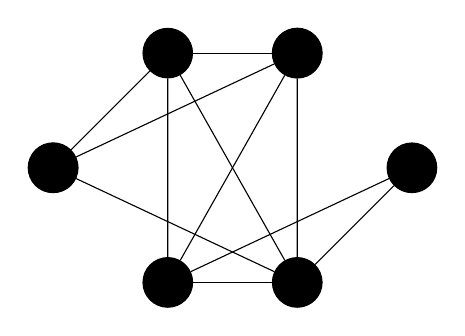
\begin{tikzpicture}[every node/.style={circle,draw=black,fill=white,black} ]
    	%\begin{tikzpicture}[every node/.style={circle,fill=DodgerBlue,white} ]
		\node(s){1};
		\node[above right=of s](a){2};
		\node[below right=of s](b){3};
		\node[right = of a](c){4};
		\node[right = of b](d){5};
		\node[below right=of c](e){6};
		
	    	
		\foreach \u / \v in{s/a,s/c,s/d,a/b,a/c,a/d,b/c,b/d,b/e,c/d,d/e}
			\draw[-] (\u)--(\v);
    	\end{tikzpicture}
	    \caption{無向グラフの例}
	    \label{fig:simplegraph}
\end{figure}  
	
	\begin{figure}[p]
	\centering
	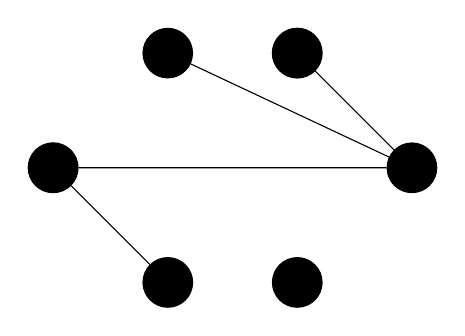
\begin{tikzpicture}[every node/.style={circle,draw=black,fill=white,black} ]
    	%\begin{tikzpicture}[every node/.style={circle,fill=DodgerBlue,white} ]
		\node(s){1};
		\node[above right=of s](a){2};
		\node[below right=of s](b){3};
		\node[right = of a](c){4};
		\node[right = of b](d){5};
		\node[below right=of c](e){6};
		
	    	
		\foreach \u / \v in{s/b,s/e,a/e,c/e}
		%\foreach \u / \v in{s/a,s/c,s/d,a/b,a/c,a/d,b/c,b/d,b/e,c/d,d/e}
			\draw[-] (\u)--(\v);
    	\end{tikzpicture}
	    \caption{図\ref{fig:simplegraph}の補グラフの例}
	    \label{fig:complementgraph}

\end{figure}


\begin{figure}[p]
\begin{tabular}{cc}
	\begin{minipage}{0.5\hsize}
	    \begin{center}
	    %\begin{tikzpicture}[every node/.style={circle,fill=DodgerBlue,white} ]
	\begin{tikzpicture}[every node/.style={circle,draw=black,fill=white,black} ]
		\node(s){1};
		\node[below right=of s](a){2};
		\node[above right=of s](b){3};
		\node[right=1.5cm of a](c){4};
		\node[right=1.5cm of b](d){5};
	    	\foreach \u / \v in{s/a,s/b,s/c,s/d,a/b,a/c,a/d,b/c,b/d,c/d}
			\draw[-] (\u)--(\v);
    	\end{tikzpicture}
	    \end{center}
	\end{minipage}
	
	\begin{minipage}{0.5\hsize}
	    \begin{center}
	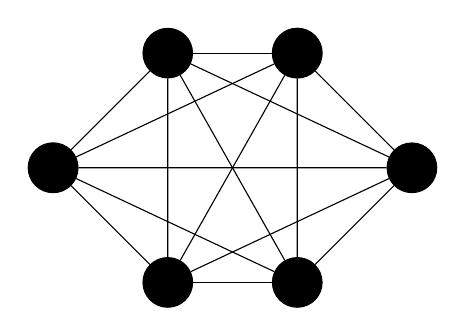
\begin{tikzpicture}[every node/.style={circle,draw=black,fill=white,black} ]
    	%\begin{tikzpicture}[every node/.style={circle,fill=DodgerBlue,white} ]
		\node(s){1};
		\node[above right=of s](a){2};
		\node[below right=of s](b){3};
		\node[right = of a](c){4};
		\node[right = of b](d){5};
		\node[below right=of c](e){6};
	    	\foreach \u / \v in{s/a,s/b,s/c,s/d,s/e,a/b,a/c,a/d,a/e,b/c,b/d,b/e,c/d,c/e,d/e}
			\draw[-] (\u)--(\v);
    	\end{tikzpicture}
	    \end{center}
	\end{minipage}
    \end{tabular}
    %\caption{完全グラフ}
    \caption{完全グラフの例}
	    \label{fig:completegraph}
	\end{figure}



\newpage
    \begin{figure}[p]
    \begin{center}
$
    \left(
	\begin{array}{cccccc}
	    0&1&0&1&1&0\\
	    1&0&1&1&1&0\\
	    0&1&0&1&1&0\\
	    1&1&1&0&1&0\\
	    1&1&1&1&0&1\\
	    0&0&1&0&1&0
	\end{array}
	\right)
$
	\caption{図\ref{fig:simplegraph}の隣接行列}
	\label{fig:Neighbormat}
    \end{center}
    \end{figure}

\begin{table}[p]
    \begin{center}
	\caption{図\ref{fig:simplegraph}の隣接リスト}
	\label{tab:nlist}
	\begin{tabular}{|c|c|}
	    \hline 
	    頂点番号& 隣接頂点\\ \hline
	    1 & 2,4,5\\ \hline
	    2 & 1,3,4,5\\ \hline
	    3 & 2,4,5,6\\ \hline
	    4 & 1,2,3,5\\ \hline
	    5 & 1,2,3,4,6\\ \hline
	    6 & 3,5 \\ \hline
	\end{tabular}
    \end{center}
\end{table}

\begin{table}[p]
    \begin{center}
	\caption{図\ref{fig:simplegraph}の補グラフの隣接リスト}
	\label{tab:nlist2}
	\begin{tabular}{|c|c|}
	    \hline 
	    頂点番号& 隣接頂点\\ \hline
	    1 & 3,6\\ \hline
	    2 & 6\\ \hline
	    3 & 1\\ \hline
	    4 & 6\\ \hline
	    5 & \\ \hline
	    6 & 1,2,4 \\ \hline
	\end{tabular}
    \end{center}
\end{table}













\chapter{既存手法}
\label{ch:prelm}

%富田らによってMCQ\cite{tomita2003efficient},MCR\cite{tomita2007efficient},MCS\cite{tomita2010simple}\cite{tomita2013simple},MCT\cite{tomita2016much}などいくつかの高速な最大クリーク抽出アルゴリズムが提案されている.
%これらのアルゴリズムは近似彩色による分枝限定法によって高速化されている.
%この章では,MCQ,MCR,MCS,MCTに共通しているアイデアについての説明をする.
%その後,本論文で提案するアルゴリズムの基になっているMCSアルゴリズムについての具体的な説明を行う.
%\section{最大クリーク抽出アルゴリズム}
%富田らによってMCQ\cite{tomita2003efficient},MCR\cite{tomita2007efficient},MCS\cite{tomita2010simple}\cite{tomita2013simple},MCT\cite{tomita2016much}などいくつかの高速な最大クリーク抽出アルゴリズムが提案されている.
%これらのアルゴリズムは近似彩色による分枝限定法によって高速化されている.
この章では, 
%Tomitaらによって提案された
%MCQと,MCR,MCS,MCTで共通して用いられている基本アイデアの深さ優先探索を\ref{sec:naive}節でナイーブアルゴリズムとして紹介する.
既存手法で用いられている深さ優先探索に基づく最大クリーク発見のアルゴリズムの説明を行う.
\ref{sec:naive}節では,厳密解を発見するナイーブアルゴリズムを与える.
\ref{sec:BB}節では,アルゴリズムを高速に動かすための改善方法について説明する.
%工夫に使われる近似彩色の基本的方法についても紹介する.
\ref{sec:MCS}節では,本論文で提案するアルゴリズムの基になっているMCSアルゴリズム\cite{tomita2010simple}\cite{tomita2013simple}について,
具体的な説明を行う.
%\subsection{ナイーブアルゴリズム}
\section{ナイーブアルゴリズム}
\label{sec:naive}
%\subsection{基本アルゴリズム}
%基本アルゴリズムとしては,ある時点で保持しているクリーク$Q$に,そのクリーク中の全ての頂点と隣接している頂点(この集合$R$を候補点集合とする)を1つ選び,
このナイーブアルゴリズムは,深さ優先探索に基づき最大クリークを求める.
ナイーブアルゴリズムの擬似コードを,Algorithm\ref{alg:BasicAlgorithm}に示す.
ある時点で保持しているクリークを$Q$,その$Q$の全ての頂点と隣接している頂点の集合を候補点集合$R$とする.
%その頂点をクリークに付け加える操作を深さ優先探索によって進めていくという手順をとる.
%このような操作を再帰的に繰り返すていくことで,候補点集合が空になったときグラフ中の極大クリークが得られる.
以下に動作を説明する.
まず,$R$の中から頂点を1つ選び$R$から取り除く.その頂点を$p$とする.$p$を$Q$に加え,$R_p$を$R$と$p$の隣接集合の積集合とする.
$R_p$を$R$としてこの操作を繰り返し行っていく.
$R$が空になったときグラフの極大クリークが得られる.
%$R$の中から頂点を1つ選びクリークに付け加える操作を行う.この操作を繰り返し行っていき,候補点集合$R$が空になったときグラフの極大クリークが得られる.
このとき得られた極大クリークのサイズが,見つかった極大クリークの中で最大のとき,それを最大クリークの候補$Q_{max}$にする.
%深さ優先探索の基本に従い,
$R$が空になった後は%1つ前の再帰処理に戻り
バックトラックをし,$Q$から$p$を削除する.
その後は,
別の頂点を選んで探索を続ける.
全ての探索が終了したときに保持している最大クリークの候補が,そのグラフの最大クリークとなる.

クリーク探索の全過程は,全頂点集合$V$を根,各時点での候補点集合$R$を頂点として,各候補点集合についての親子関係にあるものを枝で結んだ探索木として表現できる.
この探索木における枝を分枝,その総数を分枝数と呼ぶ.

\begin{algorithm}[p]
  \caption{最大クリーク抽出のナイーブアルゴリズム}
  \label{alg:BasicAlgorithm}
    \begin{algorithmic}[1]
	%\Procedure{Mc-Naive}{$G=(V,E)$}
	\Procedure{MC-NAIVE}{$G=(V,E)$}
    		\State $Q := Q_{max} := \emptyset $
		%\State \Call{Expand-Naive}{$V$}
		\State \Call{EXPAND-NAIVE}{$V$}
		\State \textbf{return} 	$Q_{max}$
	\EndProcedure
    \end{algorithmic}
    \begin{algorithmic}[1]
    %\Require $G = (V,E)$
    %\Ensure $Q_{max}$
    %\State $Q := Q_{max} := \emptyset $
	 
         \Procedure{EXPAND-NAIVE}{$R$}
         %\Procedure{Expand-Naive}{$R$}
	 	\While{ $R \neq \emptyset$ }
	 		%\State 頂点$p \in V$を1つ選ぶ
			\State $p :=$ a vertex in $R$
			\State $R := R - \{ p \} $
			\State $Q := Q \cup \{ p \} $
			\State $R_p := R \cap \{ p \} $
			\If{ $R_p \neq \emptyset$}
				\State \Call{EXPAND-NAIVE}{ $R_p$ }
				%\State \Call{Expand-Naive}{ $R_p$ }
			\ElsIf{ $Q > Q_{max}$ }
				\State $ Q_{max} := Q $
			\EndIf
			\State $Q := Q - \{ p \}$
		\EndWhile
	\EndProcedure
    \end{algorithmic} 
\end{algorithm}

\section{近似彩色による分枝限定}
\label{sec:BB}
%\subsection{近似彩色による分枝限定}
MCQ\cite{tomita2003efficient}と,MCR\cite{tomita2007efficient},MCS,MCT\cite{tomita2016much}などのアルゴリズムでは,近似彩色による分枝限定法によって
分枝数を抑えることで
高速化されている.
%これは,分枝数を抑えることで探索をより効率的に行っている.

\subsection{分枝限定法}
%\subsubsection*{分枝限定法}
アルゴリズムを高速化するためには,探索過程での分枝数を削減することが効果的である.
これを実現することが分枝限定法である.
%最大クリーク抽出の分枝限定法の一つは,

探索時に保持しているクリークを$Q$,最大クリーク候補を$Q_{max}$,候補点集合を$R$とする.
このとき,
\begin{equation}
	|Q| + |R| \leq |Q_{max}|
\notag
\end{equation}
を満たすとき,最大クリークが存在しないことは,明らかであるので探索を終了する.


%\subsection{近似彩色}
分枝限定をより効果的に適用するために彩色を利用する.
彩色とは,グラフの隣接頂点同士には異なる番号になるように番号を振ることである.
彩色の目的は,最大クリークのサイズの上界をできるだけ小さく求めることである.
%で分枝限定をより効果的にすることである.
%近似彩色の目的は,最大クリークサイズの上界をできるだけ小さく求めることで分枝限定をより効果的にすることである.
%彩色条件は,隣接する頂点同士には異なる番号で彩色することである.

\begin{lemma}[彩色による最大クリークのサイズの上界]
    グラフが隣接頂点同士には異なる番号になるように番号を振られ,彩色に使われている最大の番号を$k_{max}$とする.
    このとき,最大クリークのサイズは$k_{max}$以下になる.
    %このとき,グラフには$k_{max}$のサイズを超えるようなクリークは存在しない.
\end{lemma}
\begin{Proof*}
    グラフが彩色されときの彩色に使われた最大の番号を$k_{max}$のとき,
    最大クリークのサイズを$\omega $とする.
    %補題1が成り立たないと仮定する.次の式が成り立つ.
    %\begin{equation}
%	w > k_{max}
 %   \end{equation}
    クリークの任意の2頂点は隣り合っている.
    なので,彩色を行われると,必ずクリーク中にはクリークのサイズ以上の彩色番号$k$の頂点が存在する.
    よって,次の式が成り立つ.
    %\begin{equation}
	$ \omega \leq k \leq  k_{max}$
	%\notag
    %\end{equation}
   % \qed
  %  よって,矛盾する.
   
\end{Proof*}
頂点$p$の彩色番号を$\mathrm{No}[p]$とする.
補題1より,彩色番号の大きな頂点$p$から探索すれば,分枝限定の条件を次の式にすることができる.
\begin{equation}
	|Q| + \mathrm{No}[p] \leq | Q_{max} | 
	\notag
\end{equation}
EXPAND毎に近似彩色アルゴリズムを適用すると,
%彩色番号が大きな頂点から探索を行うことで
	上記の式を分枝条限定の条件を使うことができるので効率よく探索を終了することができる.

\subsection{近似彩色}
彩色の最適化は,NP困難に属する組合せ最適化問題であるので,近似彩色を行う
%\cite{Karp1972}
.
%以下には,
%具体的な彩色方法について述べる.
MCQとMCRで用いられている具体的な彩色方法について述べる.
彩色は,候補点集合の先頭から行い,各頂点には,隣接する頂点の頂点が持つ番号とは異なる最小の正整数を付与する.
このように,彩色を行いその番号の昇順に並べる手続きがNUMBER-SORTである.
擬似コードを,Algorithm \ref{alg:NUMBER-SORT}に示す.
$C_k$には,彩色番号$k$を持つ頂点が保存されている.
\begin{algorithm}[p]
    \caption{彩色アルゴリズム}
    \label{alg:NUMBER-SORT}

    \begin{algorithmic}[1]
	\Procedure{NUMBER-SORT}{ $R,\mathrm{No}$ }
		\State $maxno:=0 , C_1 := \emptyset$
		\While{ $R \neq \emptyset$ }
			\State $p:=$ the first vertex in $R$
			\State $k:=1$
			\While{ $C_k \cap \Gamma(p) \neq \emptyset $}
				\State $k:=k+1$
			\EndWhile
			\If{ $ k > maxno $ }
				\State $ maxno := k , C_{maxno} := \emptyset$
			\EndIf
			\State $\mathrm{No}[p] := k , C_k := C_k \cup \{p \} , R := R - \{ p \}$
		\EndWhile
		\State $i:=1$
		\For{ $k:=1$ \ \textbf{to} \ $maxno$}
			\For{ $j:=1$ \ \textbf{to} \ $|C_k|$ }
				\State $R[i] := C_k[j] , i := i+1 $
			\EndFor
		\EndFor
	\EndProcedure
    \end{algorithmic}
\end{algorithm}


%\subsubsection*{グラフの再構成}
%	キャッシュ率を上げるためにグラフの再構成を行う.

\section{MCSアルゴリズム}
\label{sec:MCS}
%\subsection{MCSアルゴリズム}
%具体的な何かを盛り込んだのかを言う
%以下の点を踏まえたのがMCSアルゴリズムである.
MCSアルゴリズムは,
\ref{sec:naive}節のナイーブアルゴリズムを基づき,後述するNUMBER-SORT-Rを彩色アルゴリズムとするアルゴリズムである.
MCSの擬似コードを,Algorithm \ref{alg:MCS_alg}に示す.
その具体的な方法について,以下で述べる.
さらに,近似解の適用によるMCSアルゴリズムの高速化についても述べる.
%MCSの擬似コードを,Algorithm \ref{alg:MCS_alg}に示す.
この節の最後には,MCSの空間計算量と時間計算量についての解析を行う.


\subsection{整列順序}
最大クリーク抽出アルゴリズムの高速化において,入力で与えられたグラフにおける初期の頂点の整列順序は重要である
\cite{富田悦次1985最大クリーク抽出の効率化手法とその実験的評価}
%\cite{}
.
%\cite{須谷洋一2006最大クリーク抽出のより高速な分枝限定アルゴリズム}.
%そのため,探索の前処理にEXTEND INITIAL SORT NUMBERを行う.
%中身をどう描くか

探索は頂点の次数の小さいものから,彩色は次数が大きなものから行うのが効率の良いかとが実験的に示されている
\cite{tomita2007efficient}
\cite{富田悦次1985最大クリーク抽出の効率化手法とその実験的評価}
.%参考文献
また,探索木の根に近い部分では,グラフに存在する最大クリークサイズと彩色番号の最大値の差が大きくなる傾向があるため彩色精度の向上による効率化が難しい.
このような場合は,次数の小さい頂点から順に探索することによる効率化を行なった方が有効な場合がある.
したがって,根の問題に限り最小次数を優先して探索することにより効率化を達成する.
最小次数の頂点が複数ある場合は,その頂点集合を$R_{min}$とし,
$ex$-$deg (p) := 
\sum_{ r \in ( R_{min} \cap \Gamma(p) ) }  deg(r) $の値が小さい順に探索を行う. 
以上のことに即した頂点の整列を探索の前処理として,初期頂点整列アルゴリズムEXTEND-INITIAL-SORT-NUMBERを行う.
EXTEND-INITIAL-SORT-NUMBERの擬似コードを,Algorithm \ref{alg:EXTEND-SORT}に示す.

\begin{algorithm}[htbp]
    \caption{初期頂点整列アルゴリズム}
    \label{alg:EXTEND-SORT}
    \small
    \begin{algorithmic}[1]
	\Procedure{EXTEND-INITIAL-SORT-NUMBER}{ $V,Q_{max} , \mathrm{No}$ }
		\State $i:=|V|$ \Comment{後ろから追加していく}
		\State $R:=V,V:=\emptyset$
		\State $R_{min}:=$ set of vertices with the minimum degree in $R$
		\While{ $| R_{min} | \neq |R| $}
			\If{ $|R_{min}| \geq 2 $}
				%\State $p:=$a vertex in $R_{min}$ such that $\sum_{r \in ( R_{min} \cap \Gamma(p) )}deg(r) = \min \{ \sum_{r \in ( R_{min} \cap \Gamma(q)  )}deg(r) \mid q \in R_{min} \}$
				\State $p:=$a vertex in $R_{min}$ such that $ex$-$deg(p) = \min \{ ex$-$deg(q) \mid q \in R_{min} \}$
			\Else \  $p := R_{min}[1]$
			\EndIf
			\State $V[i] := p , R := R - \{ p \} , i := i-1$
			\For{$j:=1$ \ \textbf{to} \ $|R|$ } \Comment{次数を直す}
				\If{ $R[j]$ is adjacent to $p$}
					\State $deg(R[j]) := deg( R[j] ) - 1 $
				\EndIf
			\EndFor
			\State $R_{min} := $set of vertices with the minimum degree in $R$
		\EndWhile
		\State \Call{ NUMBER-SORT }{ $R_{min} , \mathrm{No} $ }
		\For{ $i := 1$ \ \textbf{to} \ $|R_{min}| $ } \Comment{残りの要素を追加していく}
			\State $V[i] := R_{min}[i]$
		\EndFor
		\State $m := \max\{ \mathrm{No}[q] \mid q \in R_{min} \} $
		\If{ $m = R_{min} $ }
			\State $Q_{max} := R_{min}$
		\EndIf
		\State $m := m+1 , i:= |R_{min}| + 1$ \Comment{$|R_{min}|+1 \leq i \leq |V|$の範囲を彩色する}
		\While{ $i \leq |V| $\ \textbf{and}\ $ m \leq |V| $ }
			\State $\mathrm{No}[V[i]] := m , m:=m+1,i:=i+1$
		\EndWhile
		\While{ $ i \leq |V|$ }
			\State $\mathrm{No}[V[i]] := m ,i:=i+1$
		\EndWhile
	\EndProcedure
    \end{algorithmic}

\end{algorithm}


\subsection{再彩色アルゴリズムRE-COLOR}
%\subsubsection*{再彩色アルゴリズムRE-COLOR}
$\mathrm{No}[p] \leq | Q_{max} | - |Q| (=: cutc )$となる頂点は探索不要であるので,
この条件を満たす頂点を多くするような頂点の彩色を行いたい.
このような考えに基づき提唱されたのが,再彩色アルゴリズムRE-COLORである.
頂点$p$の彩色番号が$k$として,RE-COLORは以下の手順で行う.
%$1\leq k_1 < cutc$の範囲で,$ |\Gamma( p ) \cap C_{k_1}| = 1 $のとき,$ \{q\} = \Gamma(p) \cap C_{k_1} $として,\\
%$k_1 < k_2 < cutc $で $| \Gamma( q ) \cap C_{k_2} | = 0 $を満たすなら,\\
%頂点$p$の彩色番号を$k_1$,頂点$q$の彩色番号を$k_2$に変える.
\begin{enumerate}
    \item $1\leq k_1 < cutc$の範囲で,$ |\Gamma( p ) \cap C_{k_1}| = 1 $を満たす$k_1$を探す.
    \item $\Gamma(p) \cap C_{k_1} $の頂点を$q$とする.
    \item $k_1 < k_2 < cutc $の範囲で,$| \Gamma( q ) \cap C_{k_2} | = 0 $を満たす$k_2$を探す.
    \item 頂点$p$の彩色番号を$k_1$,$q$の彩色番号を$k_2$に変える.
\end{enumerate}

RE-COLORの動作例を図\ref{fig:RE-NUMBER}に示す.
RE-COLORの擬似コードを,Algorithm \ref{alg:Re_Color}に示す.
\begin{figure}[p]
\begin{tabular}{ccc}
%\begin{tikzpicture}[every node/.style={circle,fill=DodgerBlue,white}]
    \begin{minipage}[b]{0.3\hsize}
	\begin{center}
	\caption*{適用前}
	\scalebox{0.7}{
    \begin{tikzpicture}[every node/.style={circle,draw=black,fill=white,black} ]
		\node(s){$p$};
		\node[right =of s](a){$q$};
		\node[ above left =of s](b){};
		\node[ left = of s ](c){};
	    	\node[ below left =of s](d){};
	    	\node[ above right=of a](e){};
	    	\node[ right =of a](f){};
	    	\node[ below right=of a](g){};
		
		\begin{scope}[on background layer]
		    \node[ fit= (b) (c) (d) ,ellipse, draw=black!40 ,dashed, fill = black!10   ](h){};
		\end{scope}
		\begin{scope}[on background layer]
		    \node[ fit= (e) (f) (g) ,ellipse, draw=black!40 ,dashed, fill = black!10   ](i){};
		\end{scope}

		\node[ rectangle callout, fill = green!80 , white ,text = black, callout absolute pointer = {(h.north) }, above=2mm of h]{ \scriptsize{$k_1$でない} };
		\node[ rectangle callout, fill = green!80 , white ,text = black, callout absolute pointer = {(i.north) }, above=2mm of i]{ \scriptsize{$k_2$でない} };

		\node[draw=white,fill=white,text=black,above=1mm of s](j){$k$};
		\node[draw=white,fill=white,text=black,above=0.5mm of a](k){$k_1$};
		\foreach \u / \v in{s/a,s/b,s/c,s/d,a/e,a/f,a/g}
			\draw[-] (\u)--(\v);
\end{tikzpicture}
	}
	\end{center}
    \end{minipage}

    \begin{minipage}[b]{0.3\hsize}
	\caption*{}
	    \begin{center}
	\scalebox{0.7}{
    \begin{tikzpicture}[every node/.style={circle,draw=black,fill=white,black} ]
		\node(s){$p$};
		\node[right =of s](a){$q$};
		\node[ above left =of s](b){};
		\node[ left = of s ](c){};
	    	\node[ below left =of s](d){};
	    	\node[ above right=of a](e){};
	    	\node[ right =of a](f){};
	    	\node[ below right=of a](g){};
		
		\begin{scope}[on background layer]
		    \node[ fit= (b) (c) (d) ,ellipse, draw=black!40 ,dashed, fill =black!10   ](h){};
		\end{scope}
		\begin{scope}[on background layer]
		    \node[ fit= (e) (f) (g) ,ellipse, draw=black!40 ,dashed, fill =black!10   ](i){};
		\end{scope}

		\node[ rectangle callout, fill = green!80 , white ,text = black, callout absolute pointer = {(h.north) }, above=2mm of h]{ \scriptsize{$k_1$でない} };
		\node[ rectangle callout, fill = green!80 , white ,text = black, callout absolute pointer = {(i.north) }, above=2mm of i]{ \scriptsize{$k_2$でない} };

		\node[draw=white,fill=white,text=black,above=1mm of s](j){$k$};
		\node[draw=white,fill=white,text=black,above=0.5mm of a](k){$k_1$};
		%\node<3>[fill=white,text=R,above=1mm of s](j){$k_1$};
		%\node<3>[fill=white,text=R,above=0.5mm of a](k){$k_2$};
		\node[draw=white,fill=white,text=black,above left= of e](l){$k_2$};
		%\visible{\node[fill=white,text=black,above left= of e](l){$k_2$};}
		
		\path[-> ,every node/.style={font=\sffamily=\small} ]
		(k) edge [bend right] node [left]{}(j);
		\path[-> ,every node/.style={font=\sffamily=\small} ]
		(l) edge [bend right] node [left]{}(k);

		\foreach \u / \v in{s/a,s/b,s/c,s/d,a/e,a/f,a/g}
			\draw[-] (\u)--(\v);
	    \end{tikzpicture}
		}
	    \end{center}
    \end{minipage}
    \begin{minipage}[b]{0.3\hsize}
	\begin{center}
	\caption*{適用後}
	\scalebox{0.7}{
    \begin{tikzpicture}[every node/.style={circle,draw=black,fill=white,black} ]
		\node(s){$p$};
		\node[right =of s](a){$q$};
		\node[ above left =of s](b){};
		\node[ left = of s ](c){};
	    	\node[ below left =of s](d){};
	    	\node[ above right=of a](e){};
	    	\node[ right =of a](f){};
	    	\node[ below right=of a](g){};
		
		\begin{scope}[on background layer]
		    \node[ fit= (b) (c) (d) ,ellipse, draw=black!40 ,dashed, fill = black!10   ](h){};
		\end{scope}
		\begin{scope}[on background layer]
		    \node[ fit= (e) (f) (g) ,ellipse, draw=black!40 ,dashed, fill = black!10   ](i){};
		\end{scope}

		\node[ rectangle callout, fill = green!80 , white ,text = black, callout absolute pointer = {(h.north) }, above=2mm of h]{ \scriptsize{$k_1$でない} };
		\node[ rectangle callout, fill = green!80 , white ,text = black, callout absolute pointer = {(i.north) }, above=2mm of i]{ \scriptsize{$k_2$でない} };

		\node[draw=white,fill=white,text=black,above=1mm of s](j){$k_1$};
		\node[draw=white,fill=white,text=black,above=0.5mm of a](k){$k_2$};
		\foreach \u / \v in{s/a,s/b,s/c,s/d,a/e,a/f,a/g}
			\draw[-] (\u)--(\v);
\end{tikzpicture}
	    }
	\end{center}
    \end{minipage}
\end{tabular}
    \caption{再彩色アルゴリズムの動作}
    \label{fig:RE-NUMBER}
\end{figure}

\begin{algorithm}[p]
    \caption{再彩色アルゴリズム}
    \label{alg:Re_Color}
    \begin{algorithmic}[1]
	\Procedure{RE-COLOR}{ $p,k,cutc$ }
		\For{ $k_1 := 1 \ $ \textbf{to}$ \  cutc-1$ }
			\If{ $| C_{k_1} \cap \Gamma(p)| = 1$}
				\For{ $k_2 := k_1 \ $ \textbf{to}$ \ cutc$ }
					\If{ $| C_{k_2} \cap \Gamma(p)| = 0$}	
						\State $C_{k} := C_{k} - \{ p \} $
						\State $C_{k_1} := ( C_{k_1} - \{  q \} ) \cup \{p\}$
						\State $C_{k_2} := C_{k_2} \cup \{ q \}$
						\State \textbf{return}
					\EndIf
				\EndFor
			\EndIf
		\EndFor
	\EndProcedure
    \end{algorithmic}
\end{algorithm}


\subsection{MCSの彩色アルゴリズム}
%\subsubsection*{MCSの彩色アルゴリズム}
MCSの彩色アルゴリズムは,RE-COLORをNUMBER-SORTに組み込んだアルゴリズムである.
この彩色アルゴリズムをNUMBER-SORT-Rとする.
NUMBER-SORT-Rの擬似コードを,Algorithm \ref{alg:NUMBER_SORT_R}に示す.
彩色の順番には,探索の前処理として行われたEXTEND-INITIAL-SORT-NUMBERで並べられた初期の頂点の整列順序を用いる.
NUMBER-SORT-Rでは,頂点の整列順序に従い先頭から彩色を行う.
その頂点の彩色番号を$k$とする.
RE-COLORに時間をかけ過ぎないように,
\begin{equation}
	k > cutc かつk=(現在の最大彩色番号)
	\notag
\end{equation}
を満たすときのみ,RE-COLORを適用する.
%ある頂点$p$に対してRE-COLORの適用条件を$p$の彩色番号を$k$としたときに,
% ($k > cutc$)かつ($k=$ (現在の最大彩色番号) )であるときに限定している.
%NUMBER-SORT-Rの擬似コードを,Algorithm \ref{alg:NUMBER_SORT_R}に示す.
	
\begin{algorithm}[htbp]
    \caption{MCSの彩色アルゴリズム} 
    \small
    \label{alg:NUMBER_SORT_R}
    \begin{algorithmic}[1]
	\Procedure{ NUMBER-SORT-R }{$V_s, R , \mathrm{No} , cutc$}
		\State $|R|:=|V_s|$
		%\Statex \{NUMBER\}
		,$k_{max} :=1 $
	        ,$C_1 := \emptyset$
		\For{ $ i:=1 \ $ \textbf{to} $\ |V_s|$ }
			\State $p:=Vs[i]$,$k:=1$
			\While{ $(C_k \cap \Gamma(p) ) \neq \emptyset $}
				\State $k := k+1$
			\EndWhile
			\If{ $k > k_{max}$ }
				\State $k_{max}:=k$,$C_{k_{max}} := \emptyset$
			\EndIf
			\State $C_k := C_k \cup \{ p \} $
			%\Statex \{ == RE-COLOR適用部分 start == \}
			\If{ $ (k>cutc)$ \  \textbf{and}\  $(k = k_{max} )$ }
				\State \Call{RE-COLOR}{$p,k$}
				\If{ $C_{k_{max}} = \emptyset $ }
					\State $k_{max}:=k_{max}-1$
				\EndIf
			\EndIf
			%\Statex \{ == RE-COLOR適用部分 end== \}
		\EndFor
		%\Statex \{ SORT \}
		\State $i:=|V_s|$
		\If{ $cutc < 0 $ } 
		\State $cutc := 0$
		\EndIf
		\For{ $k:=k_{max} \ $\textbf{downto} $\ cutc+1$}
			\For{ $j:=|C_k|\ $ \textbf{downto} $\ 1$}
				\State $R[i]:=C_k[j]$
				\State $\mathrm{No}[ R[i] ]:=k$
				\State $i:=i-1$
			\EndFor
		\EndFor
		\If{ $i \neq 0$ }
			\State $\mathrm{No}[R[i]] := cutc$
		\EndIf
	\EndProcedure
    \end{algorithmic}
\end{algorithm}


\subsection{近似解の適用}
\label{sec:apply-approximate}
最大クリークの下界が既知であるのならば,従来の分枝限定法やRE-COLORの条件により探索の効率化が期待できる.
よって探索前に近似解を求めておくことで,その値を下界として探索を効率化する.
%クリーク問題については,
%一般に近似困難性が知られているため,
%多くの問題に対して良い精度を得る近似アルゴリズムは難しいが,比較的良好な近似解を得るヒューリスティックは多く存在する.
本論文の近似アルゴリズムには,\ref{sec:relation}節で紹介したKLSを利用する.
%本論文の近似アルゴリズムには,$k$-opt Local Search(KLS)\cite{katayama2005effective}を利用する.
KLSアルゴリズムとは,局所探索により最大クリークを近似するアルゴリズムである.
各探索に対して1つの頂点を起点として探索を行う.多くの頂点を起点として,
探索する回数を増やすことで近似精度の向上を期待できるが,アルゴリズムの実行時間が増加することはできるだけ避ける必要がある.
そのため,探索回数を$20\sqrt{ |V|}\times Dens( G )^3$とする.
これは,辺密度が高いグラフでは探索回数が増え,辺密度が低いグラフでは探索する頂点は少なくなる.
%\subsubsection*{MCSアルゴリズム}
%以上の点を踏まえたのがMCSアルゴリズムである.
%擬似コードはAlgorithm \ref{alg:MCS_alg}に示す.
%擬似コードをのせる.
\begin{algorithm}[htbp]
    \caption{MCSアルゴリズム}
    \small
    \label{alg:MCS_alg}
    \begin{algorithmic}[1]
	\Procedure{ MCS }{$ G = ( V ,E ) $}
		\State $Q:=\emptyset , Q_{max} := \emptyset$
		%\State 拡張イニシャルソート
		\State \Call{EXTEND-INITIAL-SORT-NUMBER}{ $ V , Q_{max} , \mathrm{No}$ }
		%\State グラフの再構成
		\State Apply approximation algorithm
		%\State \Call{EXPAND}{$V,V,\mathrm{No}$}
		\While{ $|Q| + |V| > |Q_{max}| $ }
			\State $p:=$ the last vertex in $V$
			\If{ $|Q| + \mathrm{No}[p] > |Q_{max} |$ }
				\State $V_s:= V \cap \Gamma(p)$
				\State \Call{EXPAND}{$V_s$}
			\Else \ \textbf{return} \ $Q_{max}$
			\EndIf
		\EndWhile
		%\State \Return $Q_{max}$
		\State \textbf{return} \ $Q_{max}$
	\EndProcedure
    \end{algorithmic}
    \begin{algorithmic}[1]
	\Procedure{ EXPAND }{ $ V_s $ }
		\State \Call{ NUMBER-SORT-R }{ $V_s ,R , \mathrm{No} , |Q_{max}| - |Q| $ }
		\While{ $ R \neq \emptyset $}
			\State $p:=$ the last vertex in $R$
			\If{ $ | Q | + \mathrm{No}[p] > |Q_{max} |$ }
				\State $ Q := Q \cup \{ p \}$
				\State $ V_p := V_s \cap \Gamma( p )$ \Comment{ 順序は保存する }
				\If{ $ V_p \neq \emptyset $ }
					%\State \Call{ NUMBER-SORT-R }{ $V_p , newR , \mathrm{newNo}$ }
					\State \Call{ EXPAND }{ $V_p$ }
				\ElsIf{ $|Q| > |Q_{max}| $}
					\State $Q_{max}:=Q$
				\EndIf
			\Else \  \textbf{return}
			\EndIf
			\State $Q := Q - \{ p \}$
			\State $R := R - \{ p \}$
			\State $V_s := V_s - \{ p \}$ \Comment{ 順序は保存する }
		\EndWhile
	\EndProcedure
    \end{algorithmic}
\end{algorithm}


\begin{comment}
\begin{algorithm}[htbp]
    \caption{MCSアルゴリズム}
    \label{alg:MCS_alg}
    \begin{algorithmic}[1]
	\Procedure{ MCS }{$ G = ( V ,E ) $}
		\State $Q:=\emptyset , Q_{max} := \emptyset$
		%\State 拡張イニシャルソート
		\State \Call{EXTEND-INITIAL-SORT-NUMBER}{ $ V , Q_{max}$ }
		%\State グラフの再構成
		\State Apply approximation algorithm
		\State \Call{EXPAND}{$V,V,\mathrm{No}$}
		%\State \Return $Q_{max}$
		\State \textbf{return} \ $Q_{max}$
	\EndProcedure
    \end{algorithmic}
    \begin{algorithmic}[1]
	\Procedure{ EXPAND }{ $ V_s , R , \mathrm{No} $ }
		\While{ $ R \neq \emptyset $}
			\State $p:=$ the last vertex in $R$
			\If{ $ | Q | + \mathrm{No}[p] > |Q_{max} |$ }
				\State $ Q := Q \cup \{ p \}$
				\State $ V_p := V_s \cap \Gamma( p )$ \Comment{ 順序は保存する }
				\If{ $ V_p \neq \emptyset $ }
					\State \Call{ NUMBER-SORT-R }{ $V_p , newR , \mathrm{newNo}$ }
					\State \Call{ EXPAND }{ $V_p , newR , \mathrm{newNo}$ }
				\ElsIf{ $|Q| > |Q_{max}| $}
					\State $Q_{max}:=Q$
				\EndIf
			\Else \  \textbf{return}
			\EndIf
			\State $Q := Q - \{ p \}$
			\State $R := R - \{ p \}$
			\State $V_s := V_s - \{ p \}$ \Comment{ 順序は保存する }
		\EndWhile
	\EndProcedure
    \end{algorithmic}
\end{algorithm}
\end{comment}
%\subsection{MCTアルゴリズム}
%MCT


	\begin{comment}
\begin{algorithm}[htbp]
    \caption{MCSの彩色アルゴリズム} 
    \small
    \label{alg:NUMBER_SORT_R}
    \begin{algorithmic}[1]
	\Procedure{ NUMBER-SORT-R }{$V_s, R , \mathrm{No} , cutc$}
		\State $|R|:=|V_s|$
		%\Statex \{NUMBER\}
		,$k_{max} :=1 $
	        ,$C_1 := \emptyset$
		\For{ $ i:=1 \ $ \textbf{to}$\ |V_s|$ }
			\State $p:=Vs[i]$,$k:=1$
			\While{ $(C_k \cap \Gamma(p) ) \neq \emptyset $}
				\State $k := k+1$
			\EndWhile
			\If{ $k > k_{max}$ }
				\State $k_{max}:=k$,$C_{k_{max}} := \emptyset$
			\EndIf
			\State $C_k := C_k \cup \{ p \} $
			%\Statex \{ == RE-COLOR適用部分 start == \}
			\If{ $ (k>cutc)$ \  \textbf{and}\  $(k = k_{max} )$ }
				\State \Call{RE-COLOR}{$p,k$}
				\If{ $C_{k_{max}} = \emptyset $ }
					\State $k_{max}:=k_{max}-1$
				\EndIf
			\EndIf
			%\Statex \{ == RE-COLOR適用部分 end== \}
		\EndFor
		%\Statex \{ SORT \}
		\State $i:=|V_s|$
		\If{ $cutc < 0 $ } 
		\State $cutc := 0$
		\EndIf
		\For{ $k:=k_{max} \ $\textbf{downto} $\ cutc+1$}
			\For{ $j:=|C_k|\ $ \textbf{downto}  



			$R , \mathrm{newNo}$ }
					\State \Call{ EXPAND }{ $V_p$ }
				\ElsIf{ $|Q| > |Q_{max}| $}
					\State $Q_{max}:=Q$
				\EndIf
			\Else \  \textbf{return}
			\EndIf
			\State $Q := Q - \{ p \}$
			\State $R := R - \{ p \}$
			\State $V_s := V_s - \{ p \}$ \Comment{ 順序は保存する }
		\EndWhile
	\EndProcedure
    \end{algorithmic}
\end{algorithm}

\end{comment}
\begin{comment}
\begin{algorithm}[htbp]
    \caption{MCSアルゴリズム}
    \label{alg:MCS_alg}
    \begin{algorithmic}[1]
	\Procedure{ MCS }{$ G = ( V ,E ) $}
		\State $Q:=\emptyset , Q_{max} := \emptyset$
		%\State 拡張イニシャルソート
		\State \Call{EXTEND-INITIAL-SORT-NUMBER}{ $ V , Q_{max}$ }
		%\State グラフの再構成
		\State Apply approximation algorithm
		\State \Call{EXPAND}{$V,V,\mathrm{No}$}
		%\State \Return $Q_{max}$
		\State \textbf{return} \ $Q_{max}$
	\EndProcedure
    \end{algorithmic}
    \begin{algorithmic}[1]
	\Procedure{ EXPAND }{ $ V_s , R , \mathrm{No} $ }
		\While{ $ R \neq \emptyset $}
			\State $p:=$ the last vertex in $R$
			\If{ $ | Q | + \mathrm{No}[p] > |Q_{max} |$ }
				\State $ Q := Q \cup \{ p \}$
				\State $ V_p := V_s \cap \Gamma( p )$ \Comment{ 順序は保存する }
				\If{ $ V_p \neq \emptyset $ }
					\State \Call{ NUMBER-SORT-R }{ $V_p , newR , \mathrm{newNo}$ }
					\State \Call{ EXPAND }{ $V_p , newR , \mathrm{newNo}$ }
				\ElsIf{ $|Q| > |Q_{max}| $}
					\State $Q_{max}:=Q$
				\EndIf
			\Else \  \textbf{return}
			\EndIf
			\State $Q := Q - \{ p \}$
			\State $R := R - \{ p \}$
			\State $V_s := V_s - \{ p \}$ \Comment{ 順序は保存する }
		\EndWhile
	\EndProcedure
    \end{algorithmic}
\end{algorithm}
\end{comment}
%\subsection{MCTアルゴリズム}
%MCT


\subsection{MCSアルゴリズムの空間計算量}
%MCSアルゴリズムでは,探索木の各頂点で候補点集合のサイズのメモリが必要である.
%さらに探索木の深さは最大で,クリークのサイズ$\omega$になる.
%なので,
%TomitaらによってMCSの空間計算量は,示されていないので以下にに示す.
%MCSアルゴリズムの分枝数は指数的に増加する可能性がある.よって,全体の時間計算量は指数時間である.
%グラフ$G=(V,E)$に対して,$n = |V|$,$m = |E|$とし,最大クリークのサイズを$w$とする.
%グラフ$G=(V,E)$に対して,$n$と$m$を$n = |V|$,$m = |E|$とし,最大クリークのサイズを$$とする.
%提案アルゴリズムの空間計算量に対して以下のことがいえる.
MCSは,深さ優先探索を行い,図\ref{fig:MCS}のように動作する.
したがって,MCSの空間計算量は,以下のことがいえる.
%空間計算量は$O( nw )$になる.
%よって,グラフの次数とクリークが近いとき空間計算量が大きくなりやすい.

\begin{lemma}[MCSアルゴリズムの探索中の空間計算量] 
    \label{lemma:MCS_mem}
    %最大クリークが未発見のときの
    MCSアルゴリズム探索中に使用する空間計算量は,$O(n\omega)$である.
\end{lemma}
\begin{Proof*}{}
    %基本アルゴルズムは深さ優先探索なので,
    探索の各段階で,子が探索を行っているときは,親は探索を終了できないので,候補点集合$R$やその彩色番号の情報を持っている.
    したがって,
    探索木の根から葉まで合計メモリ使用量を考える.
    探索木の子の頂点に行くときにクリーク$Q$に頂点を1つ追加しているので,探索木の最大の深さは$\omega$である.
    %探索木の各頂点では,候補点集合$R$とその彩色番号の情報を持っている.
    \begin{equation}
     |R| \leq  |V| = n 
    \notag
    \end{equation}
    したがって,探索中の空間計算量は$O(n \omega)$である.\qed
\end{Proof*}
\begin{lemma}[MCSアルゴリズムの隣接行列での空間計算量]
    MCSアルゴリズムの隣接行列での空間計算量は,$O(n^2)$である.
\end{lemma}
\begin{Proof*}{}
    MCSの探索中のに使用する空間計算量は,定理\ref{lemma:MCS_mem}から$O(n\omega)$である.
    \ref{sec:neighbormatrix}で述べたようにグラフの隣接行列の空間計算量は,$O(n^2)$である.
    $ \omega \leq m$なので,
    グラフの隣接行列でのMCSアルゴリズムの空間計算量は,
    \begin{equation}
	O( n\omega ) + O( n^2 ) = O(n^2 )
    \notag
    \end{equation}
    となる.\qed
\end{Proof*}
\begin{lemma}[MCSアルゴリズムの隣接リストでの空間計算量]
    MCSアルゴリズムの隣接リストでの空間計算量は,$O(n \omega + m )$である.
\end{lemma}

\begin{Proof*}{}
    MCSの探索中のに使用する空間計算量は,定理\ref{lemma:MCS_mem}から$O(n \omega)$である.
    %グラフの隣接行列の空間計算量は$O(n^2)$,
    \ref{sec:neighborlist}で述べたように隣接リストの空間計算量は,$O(n + m )$である.
    $\omega \leq n $なので,
    %グラフの隣接行列でのMCSアルゴリズムの空間計算量は,
    %\begin{equation}
%	O( nw ) + O( n^2 ) = O(n^2 )
 %   \end{equation}
  %  となる.\\
    グラフの隣接リストでのMCSの空間計算量は,
    \begin{equation}
    O( n\omega ) + O( n + m  ) = O( n\omega + n + m ) = O(n\omega + m )
    \notag
    \end{equation}
    となる.\qed
\end{Proof*}

\subsection{MCSアルゴリズムの時間計算量}
%TomitaらによってMCSの時間計算量は,示されていないので以下に示す.
%グラフ$G=(V,E)$に対して,$n = |V|$,$m = |E|$とする.
%グラフ$G=(V,E)$に対して,$n$と$m$を$n = |V|$,$m = |E|$とする.
%提案アルゴリズムの空間計算量に対して以下のことがいえる.
MCSの分枝数は指数的に増加する可能性がある.
したがって,全体の時間計算量は,指数時間である.
再帰処理のEXPANDにかかる時間計算量について解析をする.
\begin{lemma}[NUMBER-SORT-Rの時間計算量]
    NUMBER-SORT-Rの時間計算量は隣接行列では,$O(n^3)$時間である.
    隣接リストでは,$O(n^3 \log n )$時間である.
\end{lemma}
\begin{Proof*}{}
    %Algorithm \ref{alg:NUMBER_SORT_R}の5--7行目では,頂点$p$が彩色できる最小の彩色番号を探している.
    %これには,彩色番号$k$が付いている頂点集合$C_k$の頂点が$p$に隣接していないかを確かめる.
    %各頂点は1つしか彩色番号を持たないので,最大でも$n$回の比較しか行われない.
    %隣接行列の頂点の隣接関係を調べるのは$O(1)$時間,隣接リストでは$O( \log n )$時間で行える.
    %以上より5--7行目は,隣接行列では$O(n)$時間,隣接リストでは$O( n \log n )$時間で行える.
    Algorithm \ref{alg:NUMBER_SORT_R}の3--18行目以外は,$O(n)$時間で行える.
    3--18行目の中で最も時間がかかるのは,13行目のRE-COLORアルゴリズムである.
    隣接行列の頂点の隣接関係を調べるのは,$O(1)$時間,隣接リストでは,$O( \log n )$時間で行える.
    RE-COLORアルゴリズムの最悪な場合は,頂点$p,q$に対して全ての頂点をみる可能性があるので,
    隣接行列では,$O(n^2)$時間で隣接リストでは,$O(n^2 \log n )時間$である.
    これを,最大$n$回行う.NUMBER-SORT-Rは隣接行列では$O(n^3)$時間で行えて,隣接リストでは$O(n^3 \log n )$時間で行うことができる.
\end{Proof*}

\begin{lemma}[EXPANDの時間計算量]
    EXPANDの時間計算量は隣接行列では,$O(n^3)$時間である.
    隣接リストでは,$O(n^3 \log n)$時間である.
\end{lemma}

\begin{Proof*}{}
    %NUMBER-SORT-Rの時間計算量は$O(n^2)$である.
    Algorithm \ref{alg:MCS_alg}のEXPANDの4--17行目までの処理で再帰のEXPAND以外は,$O(n \log n)時間$で行える.
    EXPANDアルゴリズムで最も時間がかかるステップは,NUMBER-SORT-Rである.
    これを,最大で$n$回繰り返される.
    したがって,EXPANDアルゴリズムの時間計算量は隣接行列では,$O(n^3)$時間である.
    隣接リストでは,$O(n^3 \log n )$時間である.
    %NUMBER-SORT-Rは,各EXPANDの先頭処理として部分グラフを彩色していると見れる.
    %これは各EXPANDに対して一度しか行われない.
    %さらに親で行われるNUMBER-SORT-Rは子のグラフに対して行われるので,
    %EXPANDアルゴリズムの平均時間計算量は$O(n^2)$である.
\end{Proof*}


\begin{figure}[p]
\begin{tabular}{cc}
    \begin{minipage}[b]{0.5\hsize}
	    \begin{center}
    	\caption*{再帰適用前}
	    %\begin{tikzpicture}[every node/.style={circle,fill=DodgerBlue,white} ]
	\begin{tikzpicture}[every node/.style={circle,draw=black,fill=white,black} ]
	    \node[fill=black!20](s){};
		%\node(s){};
		\node[below =of s](a){};
		\node[left=of a](b){};
		\node[right =of a](c){};
		\node[ above =1mm of s , draw = white ](ss){$R$};
		\node[ above left  =1mm of b , draw = white ](cc){};
	    	\foreach \u / \v in{s/a,s/b,s/c}
			\draw[-] (\u)--(\v);
		\foreach \u / \v in{ss/cc}
			\draw[->] (\u)--(\v);	
    	\end{tikzpicture}
	    \end{center}
	\end{minipage}
	
	    \begin{minipage}[b]{0.5\hsize}
	    \begin{center}
    	\caption*{再帰適用後		
%\small{$V_{\mathrm{d}}:= R - \Gamma(p) $ }
		}
	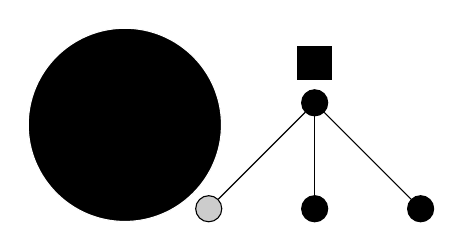
\begin{tikzpicture}[every node/.style={circle,draw=black,fill=white,black} ]
    	%\begin{tikzpicture}[every node/.style={circle,fill=DodgerBlue,white} ]
	    \node(s){};
		\node[below =of s](a){};
		\node[fill=black!20,left=of a](b){};
		\node[right =of a](c){};
		\node[rectangle , above =1mm of s , draw = white ](ss){\small{$R$} };
		\node[ above left=1mm of b , draw = white ](cc){ \small{$R':= R \cap \Gamma(p) $ } };
		%\node[above left=1mm of b , draw = white ](cc){ \small{$R':= R-V_{ \mathrm{d} }$ } };
	    	\foreach \u / \v in{s/a,s/b,s/c}
			\draw[-] (\u)--(\v);
	\end{tikzpicture}
	    \end{center}
	\end{minipage}
 \\ 
		\\
	\begin{minipage}[b]{0.5\hsize}
	    \begin{center}
    	\caption*{バックトラック適用前}
	    %\begin{tikzpicture}[every node/.style={circle,fill=DodgerBlue,white} ]
	\begin{tikzpicture}[every node/.style={circle,draw=black,fill=white,black} ]
		\node(s){};
		\node[below =of s](a){};
		\node[fill=black!20, left=of a](b){};
		\node[right =of a](c){};
		\node[ above =1mm of s , draw = white ](ss){ $R$ };
		\node[ above left  =1mm of b , draw = white ](cc){ $R'$};
		%\node[ above left  =1mm of b , draw = white ](cc){ $R'$};
	    	\foreach \u / \v in{s/a,s/b,s/c}
			\draw[-] (\u)--(\v);
		\foreach \u / \v in{ss/cc}
			\draw[<-] (\u)--(\v);	
    	\end{tikzpicture}
	    \end{center}
	\end{minipage}
	
	    \begin{minipage}[b]{0.5\hsize}
	    \begin{center}
	\caption*{バックトラック適用後
       %\small{$R := R' \cup V_{\mathrm{d} }-\{p\}$} \\  \small{$ V_{\mathrm{e} }:= V_{\mathrm{e} } \cup \{p\} $ } 
		}
	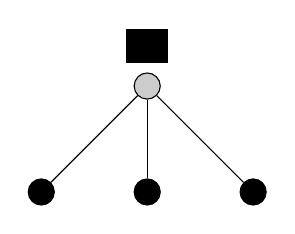
\begin{tikzpicture}[every node/.style={circle,draw=black,fill=white,black} ]
    	%\begin{tikzpicture}[every node/.style={circle,fill=DodgerBlue,white} ]
	    \node[fill=black!20](s) {};
	    %\node(s) {};
	    %\node[label=above:\small{$R:=R'\cup V_{\mathrm{d}-\{p\} } \\ V_{\mathrm{e}}:=V_{\mathrm{e}} \cup \{p\}$}  ](s) {};
		\node[below =of s](a){};
		\node[left=of a](b){};
		\node[right =of a](c){};
		%\node[above =1mm of s , draw = white ](ss){};
		%\node[ rectangle,above =1mm of s , draw = white ](ss){ \small{$R := R' \cup V_{\mathrm{d} }-\{p\} $ \newline  $ V_{\mathrm{e} }:= V_{\mathrm{e} } \cup \{p\} $ } };
		\node[ rectangle,above =1mm of s , draw = white ](ss){ \small{$R$ } };
		%\node[ rectangle,above =7mm of s , draw = white ](s2){ \small{$R := R' \cup V_{\mathrm{d} }-\{p\} $ } };
		%\node[above left=1mm of b , draw = white ](cc){};
	    	\foreach \u / \v in{s/a,s/b,s/c}
			\draw[-] (\u)--(\v);
	\end{tikzpicture}
	    \end{center}
	\end{minipage}


\end{tabular}
    %\caption{完全グラフ}
    \caption{MCSの動作  
	    }
    \label{fig:MCS}
	    \centering
	    $R,R'$は,候補点集合とし,$p$は探索を行う頂点とする.
\end{figure}





\chapter{提案手法}
\label{ch:propose}

提案する省メモリ化最大クリーク抽出アルゴリズムの概要について\ref{sec:alg-overview}節で述べる.
次にその空間計算量について\ref{sec:alg-mem}節で述べる.
最後にその時間計算量について\ref{sec:alg-time}節で述べる.


\section{アルゴリズムの概要}
\label{sec:alg-overview}
MCSアルゴリズムでは,探索中のメモリ使用量のボトルネックは,探索の各段階で持つ候補点集合の情報のサイズである.
したがって,たとえグラフを隣接リストなどで実装をしても,
グラフとクリークのサイズが大きいとき,メモリ使用量が大きくなりやすい.

提案するアルゴリズムでは,探索の各段階で持つ情報を,親から子に進むときに捨てる頂点集合のみにする.
このことで,メモリの使用量を削減するようにする.
%提案するアルゴリズムでは,探索の各段階で持つ情報を親から子に行くための差分の情報のみを保持することでメモリの使用量を削減するようにする.
%差分の情報とは,子に渡さない頂点集合のことである.それは
保持する情報には,
頂点が選ばれクリークに追加された頂点集合と頂点を追加するときに隣接しなくなった頂点集合の2種類ある.
それぞれの頂点集合を$V_\mathrm{d}$,$V_\mathrm{e}$とする.
%それぞれの頂点集合を$fix1,fix2$とする.
バックトラックするとき,その頂点集合を使用することで復元をする.
%子から親に戻る際には,その差分の情報を使用することで復元をする.
具体的な復元の仕方について,以下で説明する.
$V$の順序は,手続きEXTEND-INITIAL-SORT-NUMBERを実行した以降変化しない.
よって,適用後に頂点集合の先頭から1から頂点の番号を付け直して変える.
このことによって,
%や,
%順番を保存しておくことで
$V_\mathrm{d}$や$V_\mathrm{e}$を追加した後にソートすることで復元することができる.

たとえば,図\ref{fig:simplegraph}のグラフで,頂点$1$をクリークに追加したとする.
頂点$1$の隣接集合は,$\Gamma(1) = (2,4,5)$である.
候補点集合は,$V$から頂点$1$に隣接していない頂点を削除する.
したがって,$V' = V \cap \Gamma(1) = (2,4,5)$になりこれを子に渡す.
そして,$ V_\mathrm{d} = V-V' = ( 1,3,6 )$を保存する.
%そして,$ fix := V-V' = ( 1,3,6 )$を保存する.
このようにすることで,再帰の各段階で子に進むときに捨てる頂点集合だけを保持させて,再帰を進めることができる.
%復元するときには,まず子の頂点集合$V'$に自分が保存している子との差分の情報$fix$を追加する.
%$V = V' \cup fix = ( 2,4,5,1,3,6)$となる.
バックトラックするときの候補点集合を,復元する方法について説明する.
まず,子の頂点集合$V'$に自分が保存している頂点集合$V_\mathrm{d}$を追加する.
したがって,$V = V' \cup V_\mathrm{d} = ( 2,4,5,1,3,6)$となる.
次に,ソートすることで$V=(1,2,3,4,5,6)$となり元の配列に復元することができる.
提案アルゴリズムの動作を図\ref{fig:propose}
に示す.
提案アルゴリズムの擬似コードは,Algorithm \ref{alg:proposal}に示す.

\begin{algorithm}[p]
	\caption{提案アルゴリズム}
%\scalebox{0.9}[0.9]{
	\small
	\label{alg:proposal}
	\begin{algorithmic}[1]
	\Procedure{ MCS-PROPOSAL }{$ G = ( V ,E ) $}
		\State $Q:=\emptyset , Q_{max} := \emptyset$
		%\State 拡張イニシャルソート
		\State \Call{EXTEND-INITIAL-SORT-NUMBER}{ $ V , Q_{max} , \mathrm{No}$ }

		%\State グラフの再構成
		%\State 近似解アルゴリズムの適用
		\State Apply approximation algorithm
		\While{ $|Q| + |V| > |Q_{max}| $ }
			\State $p:=$ the last vertex in $V$
			\If{ $|Q| + \mathrm{No}[p] > |Q_{max} |$ }
				%\State $V_s:= V \cap \Gamma(p)$
				%\State \Call{EXPAND-PROPOSAL}{$V_s$}
				\State \Call{EXPAND-PROPOSAL}{$V \cap \Gamma(p)$}
			\Else \ \textbf{return} \ $Q_{max}$
			\EndIf
		\EndWhile
		%\State \Return $Q_{max}$
		\State \textbf{return} \ $Q_{max}$
	\EndProcedure
    \end{algorithmic}
    

	\begin{algorithmic}[1]
		\Procedure{ EXPAND-PROPOSAL }{ $V_s$ }
			\State $V_\mathrm{e} := \emptyset $ \Comment{一度クリークに追加された点を保存する}
			%\State $fix1 := \emptyset $ \Comment{一度クリークに追加された点を保存する}
			\While{ $V_s \neq \emptyset $}
				%\State $p:=$ the last vertex in $R$
				\State ${p,no} := $the last vertex and number in $R$ and $\mathrm{No}$ that get \Call{ NUMBER-SORT-R }{$ V_s ,R , \mathrm{No}$}
				%\State ${p,no} := $\Call{ NUMBER-SORT-R }{$ V_s ,R , \mathrm{No}$}をした結果の$R$の一番後ろの頂点とその彩色番号
				%\State $fix2 := \emptyset $ \Comment{隣接点でなく削除された点を保存する}
				\If{ $|Q| + no > |Q_{max} | $ }
					\State $ Q := Q \cup \{ p \}$
					\State $ V_\mathrm{d} :=  V_s - \Gamma(p)$ \Comment{ 隣接していないために削除された点を保存する }
					%\State $ fix2 :=  V - \Gamma(p)$ \Comment{ 隣接していないために削除された点を保存する }
					\State $ V_s := V_s \cap \Gamma(p)$
					\If{ $V_s \neq \emptyset $}
						\State \Call{ EXPAND-PROPOSAL }{ $V_s$ }
					\ElsIf{ $Q > Q_{max}$ }
						\State $Q_{max} := Q$
					\EndIf
					%\State $V,fix2$を使い元の配列に戻す
					%\State $V:=V-\{p \} , fix1 := fix1 \cup \{ p\}$
					\State $ V_s := V_s \cup V_\mathrm{d}$,sort to $V_s$ \Comment{隣接していないため削除した頂点を復元する}
					%\State $V_s$,$V_\mathrm{d}$を使い元の配列に戻す
					\State $V_s:=V_s-\{p \} , V_\mathrm{e} := V_\mathrm{e} \cup \{ p\}$
	    			\Else
					\State $V_s:= V_s \cup V_\mathrm{e}$,sort to $V_s$ \Comment{バックトラックするので,探索した頂点を復元する}
					%\State $V_s$,$V_\mathrm{e}$を使い元の配列に戻す
					%\State $V,fix1$を使い元の配列に戻す
					\State \textbf{ return }
				\EndIf
			\EndWhile
			\State $V_s := V_s \cup V_\mathrm{e}$,sort to $V_s$ \Comment{バックトラックするので,探索した頂点を復元する}

			%\State $V_s$,$V_\mathrm{e}$を使い元の配列に戻す
			%\State $V,fix1$を使い元の配列に戻す
		\EndProcedure
		
	\end{algorithmic}
\end{algorithm}

\begin{figure}[p]
\begin{tabular}{cc}
    \begin{minipage}[b]{0.5\hsize}
	    \begin{center}
    	\caption*{再帰適用前}
	    %\begin{tikzpicture}[every node/.style={circle,fill=DodgerBlue,white} ]
	\begin{tikzpicture}[every node/.style={circle,draw=black,fill=white,black} ]
	    \node[fill=black!20](s){};
		%\node(s){};
		\node[below =of s](a){};
		\node[left=of a](b){};
		\node[right =of a](c){};
		\node[ above =1mm of s , draw = white ](ss){$R$};
		\node[ above left  =1mm of b , draw = white ](cc){};
	    	\foreach \u / \v in{s/a,s/b,s/c}
			\draw[-] (\u)--(\v);
		\foreach \u / \v in{ss/cc}
			\draw[->] (\u)--(\v);	
    	\end{tikzpicture}
	    \end{center}
	\end{minipage}
	
	    \begin{minipage}[b]{0.5\hsize}
	    \begin{center}
    	\caption*{再帰適用後		
%\small{$V_{\mathrm{d}}:= R - \Gamma(p) $ }
		}
	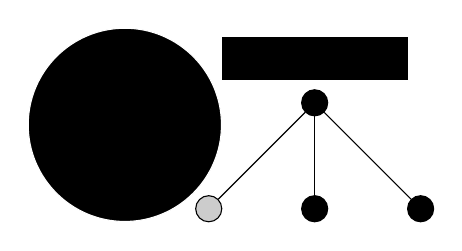
\begin{tikzpicture}[every node/.style={circle,draw=black,fill=white,black} ]
    	%\begin{tikzpicture}[every node/.style={circle,fill=DodgerBlue,white} ]
	    \node(s){};
		\node[below =of s](a){};
		\node[fill=black!20,left=of a](b){};
		\node[right =of a](c){};
		\node[rectangle , above =1mm of s , draw = white ](ss){\small{$V_{\mathrm{d}} := R - \Gamma(p)$} };
		\node[ above left=1mm of b , draw = white ](cc){ \small{$R':= R \cap \Gamma(p)$ } };
		%\node[above left=1mm of b , draw = white ](cc){ \small{$R':= R-V_{ \mathrm{d} }$ } };
	    	\foreach \u / \v in{s/a,s/b,s/c}
			\draw[-] (\u)--(\v);
	\end{tikzpicture}
	    \end{center}
	\end{minipage}
 \\ 
		\\
	\begin{minipage}[b]{0.5\hsize}
	    \begin{center}
    	\caption*{バックトラック適用前}
	    %\begin{tikzpicture}[every node/.style={circle,fill=DodgerBlue,white} ]
	\begin{tikzpicture}[every node/.style={circle,draw=black,fill=white,black} ]
		\node(s){};
		\node[below =of s](a){};
		\node[fill=black!20, left=of a](b){};
		\node[right =of a](c){};
		\node[ above =1mm of s , draw = white ](ss){ $V_{ \mathrm{d} }$ };
		\node[ above left  =1mm of b , draw = white ](cc){ $R'$};
		%\node[ above left  =1mm of b , draw = white ](cc){ $R'$};
	    	\foreach \u / \v in{s/a,s/b,s/c}
			\draw[-] (\u)--(\v);
		\foreach \u / \v in{ss/cc}
			\draw[<-] (\u)--(\v);	
    	\end{tikzpicture}
	    \end{center}
	\end{minipage}
	
	    \begin{minipage}[b]{0.5\hsize}
	    \begin{center}
	\caption*{バックトラック適用後
       %\small{$R := R' \cup V_{\mathrm{d} }-\{p\}$} \\  \small{$ V_{\mathrm{e} }:= V_{\mathrm{e} } \cup \{p\} $ } 
		}
	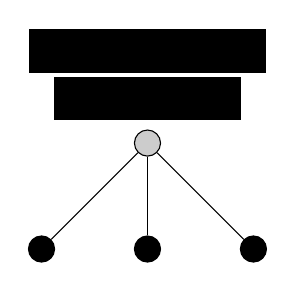
\begin{tikzpicture}[every node/.style={circle,draw=black,fill=white,black} ]
    	%\begin{tikzpicture}[every node/.style={circle,fill=DodgerBlue,white} ]
	    \node[fill=black!20](s) {};
	    %\node(s) {};
	    %\node[label=above:\small{$R:=R'\cup V_{\mathrm{d}-\{p\} } \\ V_{\mathrm{e}}:=V_{\mathrm{e}} \cup \{p\}$}  ](s) {};
		\node[below =of s](a){};
		\node[left=of a](b){};
		\node[right =of a](c){};
		%\node[above =1mm of s , draw = white ](ss){};
		%\node[ rectangle,above =1mm of s , draw = white ](ss){ \small{$R := R' \cup V_{\mathrm{d} }-\{p\} $ \newline  $ V_{\mathrm{e} }:= V_{\mathrm{e} } \cup \{p\} $ } };
		\node[ rectangle,above =1mm of s , draw = white ](ss){ \small{$ V_{\mathrm{e} }:= V_{\mathrm{e} } \cup \{p\} $ } };
		\node[ rectangle,above =7mm of s , draw = white ](s2){ \small{$R := R' \cup V_{\mathrm{d} }-\{p\} $ } };
		%\node[above left=1mm of b , draw = white ](cc){};
	    	\foreach \u / \v in{s/a,s/b,s/c}
			\draw[-] (\u)--(\v);
	\end{tikzpicture}
	    \end{center}
	\end{minipage}


\end{tabular}
	  %  \begin{center}
    %\caption{完全グラフ}
    \caption{
	提案手法の動作
	    %$V_{\mathrm{d}}$は,各再帰で隣接していないので捨てる頂点集合とする.\\
	    %$V_{\mathrm{e}}$は,各再帰の探索済みの頂点の集合とする.
	    }
    \label{fig:propose}
	   \centering
	    $R,R'$は,候補点集合とし,$p$は探索を行う頂点とする.
	      $V_{\mathrm{d}}$は,各再帰で隣接していないので,子に持たせない頂点集合とする.
	      $V_{\mathrm{e}}$は,各再帰の探索済みの頂点の集合とする.
	   % \end{center}
\end{figure}





\begin{comment}
\begin{algorithm}[p]
	\caption{提案アルゴリズム}
	\small
	\label{alg:proposal}
	\begin{algorithmic}[1]
	\Procedure{ MCS-PROPOSAL }{$ G = ( V ,E ) $}
		\State $Q:=\emptyset , Q_{max} := \emptyset$
		%\State 拡張イニシャルソート
		\State \Call{EXTEND-INITIAL-SORT-NUMBER}{ $ V , Q_{max} , No$ }
		%\State グラフの再構成
		%\State 近似解アルゴリズムの適用
		\State Apply approximation algorithm
		\State \Call{EXPAND-PROPOSAL}{$V$}
		%\State \Return $Q_{max}$
		\State \textbf{return} \ $Q_{max}$
	\EndProcedure
    \end{algorithmic}

	\begin{algorithmic}[1]
		\Procedure{ EXPAND-PROPOSAL }{ $V_s$ }
			\State $ cutc:= |Q_{max}| -|Q|$
			\State $V_\mathrm{e} := \emptyset $ \Comment{一度クリークに追加された点を保存する}
			%\State $fix1 := \emptyset $ \Comment{一度クリークに追加された点を保存する}
			\While{ $V_s \neq \emptyset $}
				%\State $p:=$ the last vertex in $R$
				\State ${p,no} := $\Call{ NUMBER-SORT-R }{$ V_s ,R , No,cutc$}をした結果の$R$の一番後ろの頂点とその彩色番号
				%\State $fix2 := \emptyset $ \Comment{隣接点でなく削除された点を保存する}
				\If{ $|Q| + no > |Q_{max} | $ }
					\State $ Q := Q \cup \{ p \}$
					\State $ V_\mathrm{d} :=  V_s - \Gamma(p)$ \Comment{ 隣接していないために削除された点を保存する }
					%\State $ fix2 :=  V - \Gamma(p)$ \Comment{ 隣接していないために削除された点を保存する }
					\State $ V_s := V_s \cap \Gamma(p)$
					\If{ $V \neq \emptyset $}
						\State \Call{ EXPAMD-proposal }{ $V_s$ }
					\ElsIf{ $Q > Q_{max}$ }
						\State $Q_{max} := Q$
					\EndIf
					%\State $V,fix2$を使い元の配列に戻す
					%\State $V:=V-\{p \} , fix1 := fix1 \cup \{ p\}$
					\State $V_s$,$V_\mathrm{d}$を使い元の配列に戻す
					\State $V_s:=V_s-\{p \} , V_\mathrm{e} := V_\mathrm{e} \cup \{ p\}$
	    			\Else
					\State $V_s$,$V_\mathrm{e}$を使い元の配列に戻す
					%\State $V,fix1$を使い元の配列に戻す
					\State \textbf{ return }
				\EndIf
			\EndWhile
			\State $V_s$,$V_\mathrm{e}$を使い元の配列に戻す
			%\State $V,fix1$を使い元の配列に戻す
		\EndProcedure
		
	\end{algorithmic}
\end{algorithm}
\end{comment}

\begin{comment}
\begin{figure}[p]
\begin{tabular}{ccc}
    \begin{minipage}[b]{0.33\hsize}
	    \begin{center}
    	\caption*{適用前}
	    %\begin{tikzpicture}[every node/.style={circle,fill=DodgerBlue,white} ]
	\begin{tikzpicture}[every node/.style={circle,draw=black,fill=white,black} ]
		\node(s){};
		\node[above =3mm of s , draw = white ](ss){$R$};
		\node[below =of s](a){};
		\node[left=of a](b){};
		\node[right =of a](c){};
		\node[above left=1mm of b , draw = white ](cc){};
	    	\foreach \u / \v in{s/a,s/b,s/c}
			\draw[-] (\u)--(\v);
		\foreach \u / \v in{ss/cc}
			\draw[->] (\u)--(\v);	
    	\end{tikzpicture}
	    \end{center}
	\end{minipage}
		
	\begin{minipage}[b]{0.33\hsize}
	    \begin{center}
    	\caption*{MCS再帰適用後}
	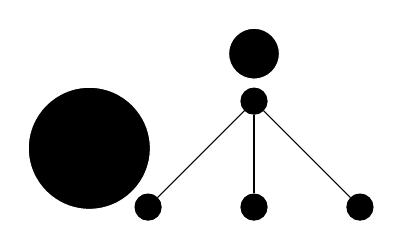
\begin{tikzpicture}[every node/.style={circle,draw=black,fill=white,black} ]
    	%\begin{tikzpicture}[every node/.style={circle,fill=DodgerBlue,white} ]
	    \node(s){};
		\node[below =of s](a){};
		\node[left=of a](b){};
		\node[right =of a](c){};
		\node[above =1mm of s , draw = white ](ss){\small{$R$}};
		\node[above left=1mm of b , draw = white ](cc){\small{$R\cap \Gamma(p)$}};
	    	\foreach \u / \v in{s/a,s/b,s/c}
			\draw[-] (\u)--(\v);
	\end{tikzpicture}
	    \end{center}
	\end{minipage}



	    \begin{minipage}[b]{0.33\hsize}
	    \begin{center}
    	\caption*{提案手法再帰適用後}
	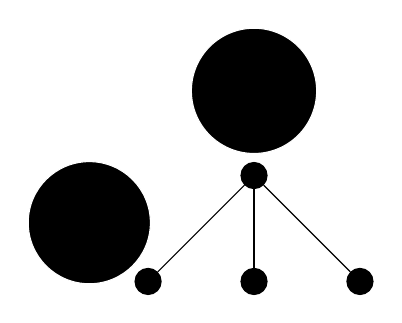
\begin{tikzpicture}[every node/.style={circle,draw=black,fill=white,black} ]
    	%\begin{tikzpicture}[every node/.style={circle,fill=DodgerBlue,white} ]
	    \node(s){};
		\node[below =of s](a){};
		\node[left=of a](b){};
		\node[right =of a](c){};
		\node[above =1mm of s , draw = white ](ss){\small{$R-\Gamma(p)$}};
		\node[above left=1mm of b , draw = white ](cc){\small{$R\cap \Gamma(p)$}};
	    	\foreach \u / \v in{s/a,s/b,s/c}
			\draw[-] (\u)--(\v);
	\end{tikzpicture}
	    \end{center}
	\end{minipage}

\end{tabular}
    %\caption{完全グラフ}
    \caption{子に進む動作}
    \label{fig:child}
	
\end{figure}

\begin{figure}[p]
\begin{tabular}{cc}
    \begin{minipage}[b]{0.5\hsize}
	    \begin{center}
    	\caption*{バックトラック適用前}
	    %\begin{tikzpicture}[every node/.style={circle,fill=DodgerBlue,white} ]
	\begin{tikzpicture}[every node/.style={circle,draw=black,fill=white,black} ]
		\node(s){};
		\node[below =of s](a){};
		\node[left=of a](b){};
		\node[right =of a](c){};
		\node[ above =1mm of s , draw = white ](ss){\small{$R-\Gamma(p)$} };
		\node[ above left  =1mm of b , draw = white ](cc){\small{$R\cap \Gamma(p)$}};
	    	\foreach \u / \v in{s/a,s/b,s/c}
			\draw[-] (\u)--(\v);
		\foreach \u / \v in{ss/cc}
			\draw[<-] (\u)--(\v);	
    	\end{tikzpicture}
	    \end{center}
	\end{minipage}
	
	    \begin{minipage}[b]{0.5\hsize}
	    \begin{center}
    	\caption*{バックトラック適用後}
	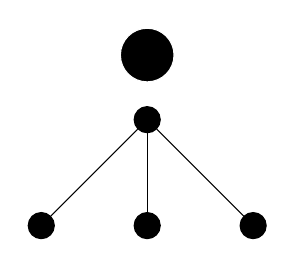
\begin{tikzpicture}[every node/.style={circle,draw=black,fill=white,black} ]
    	%\begin{tikzpicture}[every node/.style={circle,fill=DodgerBlue,white} ]
	    \node(s){};
		\node[below =of s](a){};
		\node[left=of a](b){};
		\node[right =of a](c){};
		\node[above =3mm of s , draw = white ](ss){$R$};
		%\node[above =3mm of b , draw = white ](cc){};
	    	\foreach \u / \v in{s/a,s/b,s/c}
			\draw[-] (\u)--(\v);
	\end{tikzpicture}
	    \end{center}
	\end{minipage}

\end{tabular}
    %\caption{完全グラフ}
    \caption{提案手法でのバックトラック動作}
    \label{fig:child}
	
\end{figure}

\begin{figure}[p]
\begin{tabular}{cc}
    \begin{minipage}[b]{0.5\hsize}
	    \begin{center}
    	\caption*{再帰適用前}
	    %\begin{tikzpicture}[every node/.style={circle,fill=DodgerBlue,white} ]
	\begin{tikzpicture}[every node/.style={circle,draw=black,fill=white,black} ]
		\node(s){};
		\node[below =of s](a){};
		\node[left=of a](b){};
		\node[right =of a](c){};
		\node[ above =1mm of s , draw = white ](ss){$R$};
		\node[ above left  =1mm of b , draw = white ](cc){};
	    	\foreach \u / \v in{s/a,s/b,s/c}
			\draw[-] (\u)--(\v);
		\foreach \u / \v in{ss/cc}
			\draw[->] (\u)--(\v);	
    	\end{tikzpicture}
	    \end{center}
	\end{minipage}
	
	    \begin{minipage}[b]{0.5\hsize}
	    \begin{center}
    	\caption*{再帰適用後		
%\small{$V_{\mathrm{d}}:= R - \Gamma(p) $ }
		}
	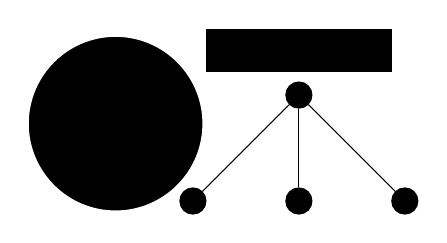
\begin{tikzpicture}[every node/.style={circle,draw=black,fill=white,black} ]
    	%\begin{tikzpicture}[every node/.style={circle,fill=DodgerBlue,white} ]
	    \node(s){};
		\node[below =of s](a){};
		\node[left=of a](b){};
		\node[right =of a](c){};
		\node[rectangle , above =1mm of s , draw = white ](ss){\small{$V_{\mathrm{d}} := R - \Gamma(p)$} };
		\node[above left=1mm of b , draw = white ](cc){ \small{$R':= R-V_{ \mathrm{d} }$ } };
	    	\foreach \u / \v in{s/a,s/b,s/c}
			\draw[-] (\u)--(\v);
	\end{tikzpicture}
	    \end{center}
	\end{minipage}
 \\ 
		\\
	\begin{minipage}[b]{0.5\hsize}
	    \begin{center}
    	\caption*{バックトラック適用前}
	    %\begin{tikzpicture}[every node/.style={circle,fill=DodgerBlue,white} ]
	\begin{tikzpicture}[every node/.style={circle,draw=black,fill=white,black} ]
		\node(s){};
		\node[below =of s](a){};
		\node[left=of a](b){};
		\node[right =of a](c){};
		\node[ above =1mm of s , draw = white ](ss){ $V_{ \mathrm{d} }$ };
		\node[ above left  =1mm of b , draw = white ](cc){ $R'$};
	    	\foreach \u / \v in{s/a,s/b,s/c}
			\draw[-] (\u)--(\v);
		\foreach \u / \v in{ss/cc}
			\draw[<-] (\u)--(\v);	
    	\end{tikzpicture}
	    \end{center}
	\end{minipage}
	
	    \begin{minipage}[b]{0.5\hsize}
	    \begin{center}
	\caption*{バックトラック適用後
       %\small{$R := R' \cup V_{\mathrm{d} }-\{p\}$} \\  \small{$ V_{\mathrm{e} }:= V_{\mathrm{e} } \cup \{p\} $ } 
		}
	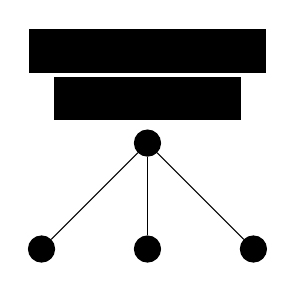
\begin{tikzpicture}[every node/.style={circle,draw=black,fill=white,black} ]
    	%\begin{tikzpicture}[every node/.style={circle,fill=DodgerBlue,white} ]
	    \node(s) {};
	    %\node[label=above:\small{$R:=R'\cup V_{\mathrm{d}-\{p\} } \\ V_{\mathrm{e}}:=V_{\mathrm{e}} \cup \{p\}$}  ](s) {};
		\node[below =of s](a){};
		\node[left=of a](b){};
		\node[right =of a](c){};
		%\node[above =1mm of s , draw = white ](ss){};
		%\node[ rectangle,above =1mm of s , draw = white ](ss){ \small{$R := R' \cup V_{\mathrm{d} }-\{p\} $ \newline  $ V_{\mathrm{e} }:= V_{\mathrm{e} } \cup \{p\} $ } };
		\node[ rectangle,above =1mm of s , draw = white ](ss){ \small{$ V_{\mathrm{e} }:= V_{\mathrm{e} } \cup \{p\} $ } };
		\node[ rectangle,above =7mm of s , draw = white ](s2){ \small{$R := R' \cup V_{\mathrm{d} }-\{p\} $ } };
		%\node[above left=1mm of b , draw = white ](cc){};
	    	\foreach \u / \v in{s/a,s/b,s/c}
			\draw[-] (\u)--(\v);
	\end{tikzpicture}
	    \end{center}
	\end{minipage}


\end{tabular}
    %\caption{完全グラフ}
    \caption{提案手法の動作\\
	    }
    \label{fig:child}
	
\end{figure}



\end{comment}



\section{アルゴリズムの空間計算量}
\label{sec:alg-mem}
%提案アルゴリズムの空間計算量は,探索木の頂点は子との差分の情報のみ保持するので探索木の根から自分までの各段階の合計で$O(n)$のメモリを使用する.

%グラフ$G=(V,E)$に対して,$n$と$m$を$n = |V|$,$m = |E|$とする.
提案アルゴリズムの空間計算量に対して,以下のことがいえる.
\begin{theorem}[提案アルゴリズムの探索中の空間計算量]
    \label{theorem:propose_mem}
    提案アルゴリズム探索中に使用する空間計算量は,$O(n)$ である.
\end{theorem}
\begin{Proof*}{}
  %  探索木の各頂点は子との差分の情報のみ保持しているので
    EXPAND-PROPOSALでは,保持する主なデータは,$V_\mathrm{e}$,$V_\mathrm{d}$である.
   これは子との差分の情報なので,
    探索木の根からどの探索の段階までの合計もグラフの頂点集合のサイズを超えない.
    したがって,探索中に使用するの空間計算量は,$O(n)$となる.
\qed
\end{Proof*}
\begin{theorem}[提案アルゴリズムの隣接行列の空間計算量]
    提案アルゴリズムの隣接行列の空間計算量は,$O(n^2)$である.
\end{theorem}

\begin{Proof*}{}
    提案アルゴリズムの探索中に使用する空間計算量は,定理\ref{theorem:propose_mem}から$O(n)$である.
    \ref{sec:neighbormatrix}で述べたようにグラフの隣接行列の空間計算量は,$O(n^2)$である.
    グラフの隣接行列での提案アルゴリズムの空間計算量は,
    \begin{equation}
	O( n ) + O( n^2 ) = O(n^2 )
    \notag
    \end{equation}
    となる.
\qed
\end{Proof*}


\begin{theorem}[提案アルゴリズムの隣接リストの空間計算量]
    提案アルゴリズムの隣接リストでの空間計算量は,$O(n + m )$である.
\end{theorem}

\begin{Proof*}{}
    提案アルゴリズムの探索中に使用する空間計算量は,定理\ref{theorem:propose_mem}から$O(n)$である.
    %グラフの隣接行列の空間計算量は$O(n^2)$,
    \ref{sec:neighborlist}で述べたようにグラフの隣接リストの空間計算量は,$O(n + m )$である.
    %グラフの隣接行列での提案アルゴリズムの空間計算量は,
    %\begin{equation}
%	O( n ) + O( n^2 ) = O(n^2 )
 %   \end{equation}
  %  となる.\\
    グラフの隣接リストでの提案アルゴリズムの空間計算量は,
    \begin{equation}
    O( n ) + O( n + m ) = O( n + n + m) = O(n + m )
    \notag
    \end{equation}
    となる.
\qed
\end{Proof*}

\section{アルゴリズムの時間計算量}
\label{sec:alg-time}
%従来のMCSアルゴリズムでは,各段階で彩色アルゴリズムNUMBER-SORT-Rを一度だけ行うが,
%提案手法では,自分の子の数だけ行われる.
%これは,かなり悪化するように考えられそうだが,子が自分に来るためにNUMBER-SORT-Rを行われるとみれば行われるのは一度だけで,
%各段階での時間計算量は,自分に対するNUMBER-SORT-Rする時間計算量から親のNUMBER-SORT-Rする時間計算量の差と差分の情報からの復元が従来のアルゴリズムより増えていると考えられる.
%グラフ$G=(V,E)$で$n = |V|$,$m = |E|$とする.
%グラフ$G=(V,E)$に対して,$n$と$m$を$n = |V|$,$m = |E|$とする.
提案アルゴリズムの空間計算量に対して,以下のことがいえる.
提案アルゴリズムの分枝数は,指数的に増加する可能性がある.
したがって,全体の時間計算量は,指数時間である.
提案アルゴリズムの分枝の処理EXPAND-PROPOSALの時間計算量についても解析をする.

\begin{theorem}[EXPAND-PROPOSALの時間計算量]
    EXPAND-PROPOSALの時間計算量は隣接行列では,$O(n^4)$時間で,
    隣接リストでは,$O(n^4 \log n )$時間である.
\end{theorem}

\begin{Proof*}
    Algorithm \ref{alg:proposal}のEXPAND-PROPOSALの5--19行のEXPAND-PROPOSALを以外の処理と3--20行以外の処理は$O(n\log n)$で全て行うことができる.
    3--20行のループで最も時間がかかる処理は,4行目の処理である.
    ループの回数は,最大で$n$回行う.
    したがって,EXPAND-PROPOSALの時間計算量は隣接行列では,$O(n^4)$時間で,隣接リストでは,$O(n^4\log n )$である.
\end{Proof*}

\begin{comment}
\begin{theorem}
    EXPAND-PROPOSALの時間計算量は,$O(n^3)$である.
    EXPAND-PROPOSALのを受け渡した親の部分グラフのサイズを$n_p$とすると,平均時間計算量は,$O(n_p^2)$である.
\end{theorem}
\begin{Proof*}
    NUMBER-SORT-Rの時間計算量は,$O(n^2)$である.
    EXPAND-PROPOSALのAlgorithm\ref{alg:proposal}の3--19行目までの処理で再帰のEXPAND-PROPOSALとNUMBER-SORT-R以外は,$O(n\log n)$で行える.
    EXPAND-PROPOSALアルゴリズムで最も時間がかかるステップは,NUMBER-SORT-Rである.
    これを最大で$n$回繰り返される.
    したがって,EXPAND-PROPOSALアルゴリズムの時間計算量は,$O(n^3)$である.
    %NUMBER-SORT-Rは,EXPANDに対して一度しか行われない,
    各EXPANDに対して,NUMBER-SORT-Rは部分問題の子の数と分枝限定の条件で停止する1回分だけ行われる.
    NUMBER-SORT-Rは,各EXPAND-PROPOSALの先頭処理として部分グラフを彩色していると見れる.
    EXPAND-PROPOSALに対して,親サイズのNUMBER-SORT-Rと分枝限定の条件を確認するための2回行われると考えられる.
    ただし,NUMBER-SORT-Rは親のサイズで行われているのでEXPAND-PROPOSALアルゴリズムの平均時間計算量は$O(n_p^2)$である.

\end{Proof*}
\end{comment}

\begin{comment}
%平均的にみると自分の部分グラフのサイズと親の部分グラフのサイズの差の分だけ時間計算量が悪化する.
時間計算量をみるとMCSのEXPANDに比べてかなり悪化しているようにみえるが,
EXPAND-PROPOSALでのNUMBER-SORT-Rは,子に進むためと分枝条件で止まるのためにしか行われない.
このため,NUMBER-SORT-Rは最大でも全体で分枝数の2倍の回数しか行われない.
MCSではNUMBER-SORT-Rは分枝数と同じ回数行うので,提案手法はMCSに対して大きく悪化することはないと考える.

\end{comment}


\chapter{実験}
\label{ch:ex}

提案アルゴリズムがMCSに対して,
最大メモリ使用量と実行時間がどれだけ増減するのかを確認するために実験を行う.
さらに,再帰処理の回数の分枝数や彩色アルゴリズムNUMBER-SORT-Rの実行回数が,実行時間に大きく関わっていると考えられるので,それらの回数も調べる.%
%さらに実行時間には,再帰処理の回数の分枝数や彩色アルゴリズムNUMBER-SORT-Rの実行回数が大きく関わると考えられるためその回数も調べる.%
また,以上の結果に対して考察を行う.
\section{実験方法}
実験方法としては,MCSと提案アルゴリズムを以下の条件に分けて実験を行った.
グラフのデータ構造については,隣接行列と隣接リスト
の2通りについて用意した.
辺密度が大きなグラフを多く扱ったので,補グラフでグラフを持つようにした.
近似解のアルゴリズムについては,適用をする場合と適用しない場合の2通りについて用意した.
計4通りの条件を,MCSと提案アルゴリズムのそれぞれに対して行った.
近似解は,\ref{sec:apply-approximate}で述べたKLSアルゴリズムによって得られた解のことする.
実験に使用したグラフは,DIMACSベンチマークセットのグラフ\footnote{\url{http://iridia.ulb.ac.be/~fmascia/maximum_clique/DIMACS-benchmark}}
とクリークサイズの大きなグラフから辺をいくつか削除することで作成したグラフ, 
DIMACSのグラフのいくつかのグラフを合体させて,そのグラフ間に辺をランダムに引くことによって作成したグラフ
の3種類を用意した.
クリークサイズの大きなグラフを作るため,完全グラフから辺をいくつか削除したグラフは2000-1500のように「$a$-$b$」のような名前で表す.
「$a$-$b$」は,グラフサイズ$a$の完全グラフから$b$本の辺を削除したグラフである.
DIMACSを合体させたグラフは,unionとunion2の2つである.unionは,c-fat200-1とMANNa-45のグラフを組み合わせたものである.
union2は,c-fat200-1と,MANNa-45,hamming10-2を組み合わせたものである.

実験環境は,
Intel Core i5-7360U CPU
(クロック周波数 : 2.30GHz,
L2 Cached : 256 KB,
L3 Cached : 4 MB
)
,主メモリ8 GB のMacOSver.10.14.6のPC上で,全てのプログラムは,gcc 8.3.0 -O3 -lm でコンパイルを行った.


\section{結果と考察}
%\section{結果}
MCS手法において,近似なし隣接行列をMCS$_{0m}$,近似なし隣接リストをMCS$_{0l}$,近似あり隣接行列をMCS$_{m}$,近似あり隣接リストをMCS$_{l}$とする.
また,提案手法において,近似なし隣接行列をMCSP$_{0m}$,近似なし隣接リストをMCSP$_{0l}$,近似あり隣接行列をMCSP$_{m}$,近似あり隣接リストをMCSP$_{l}$とする.

実行時間と,最大メモリ使用量,分枝数とNUMBER-SORT-Rの実行回数の結果を表\ref{tab:result_sec} ,表\ref{tab:result_mem},表\ref{tab:result_num}に示す.
failは,実行に失敗したことを示す.
各グラフに対して,時間が最も速いものと最大メモリ使用量が最も小さいものは,太字で示している.
NSR数は,NUMBER-SORT-Rの実行回数のことを示している.
%\section{考察}
以下では,結果の比較と考察を行う.

\subsection{MCSと提案手法の比較}
提案アルゴリズムは,MCSに対して実行時間では,2から4倍程度悪化するものが多かった.
分枝数は,MCSと提案手法で大きな差がなかった.
これは,同じ彩色アルゴリズムを適用しているため,ほぼ同じ探索をしたからだと考えられる.
分枝数の僅かな差は,NUMBER-SORT-Rを繰り返し適用しているので,
RE-COLORが適用される頂点が増えるために僅かに分枝数が減少したと考察する.
NUMBER-SORT-Rの実行回数は,
MCSの彩色は,再帰の前処理としてのみしか行われないため,
MCSでは分枝数以下の回数しか行われなかった.
また,提案アルゴリズムでは分枝数の2倍以下の回数しか行われなかった.
これは,提案アルゴリズムの彩色は,子の再帰の前処理と再帰の終了の条件のためにしか行われないため,
全体として分枝数の2倍以下しか行われなかったと考察をする.
MCSでの時間計算量が隣接行列で$O(n^3)$時間,隣接リストで$O(n^3 \log n )$時間で,
提案アルゴリズムでの時間計算量が隣接行列で$O(n^4)$時間,隣接リストで$O(n^4 \log n )$時間である.
提案アルゴリズムの時間計算量がMCSに対して大きく増加しているのに,
実行時間が2から4倍程度に抑えられているのは,
分枝数に大きな増加がないことや提案アルゴリズムの彩色の適用回数が分枝数の2倍以下であること
によるためだと考察する.

解のサイズが大きなグラフに対しては,最大メモリ使用量の減少が確認できた.
しかし,解のサイズが小さなものにはほとんど効果が見受けられなかった.
%これは,探索中に使用する空間計算量がMCSアルゴリズムでは$O(nw)$で,提案手法では,$O(n)$ で$w$が小さいときはこの差が小さくなるからであると考察する.%補題定理を引く
これは,MCSの探索木の深さが大きくないときMCSのメモリ使用量も大きくならず,
探索木の深さの最大値は,最大クリークのサイズに等しいからだであると考察する.

failで表したように実行ができなかったものは,完全グラフから辺をいくつか削除して作られたグラフである.
これはクリークサイズが大きいので,近似解を用いない方法では,提案アルゴリズムでなければメモリ使用量が大きくなるため,
スタック領域が足りなくなり動かなかったと考える.
\subsection{隣接行列と隣接リストの比較}
実行時間は,隣接リストの方が,隣接行列に比べて3から10倍程度悪くなった.
隣接リストが,隣接行列よりある頂点$p$の隣接関係を調べるのに,$O(\log | \Gamma(p) |)$倍かかるために実行時間が悪化したと考察する.
%隣接行列が隣接リストよりある頂点$p$の隣接関係を調べるのに,$O(\log | \Gamma(p) |)$倍かかるために実行時間が悪化したと考察する.

最大メモリ使用量は,隣接リストは隣接行列に比べて,
辺密度がある程度大きいものはほとんどが最大メモリ使用量が小さくなったが,
辺密度が小さいものは,メモリ使用量が増加した.
隣接リストを補グラフで保持しているので,
辺密度が小さいとき保持するデータが多くなるため,最大メモリ使用量が隣接行列で保持するより大きくなったと考察する.

\subsection{近似アルゴリズムの適用する場合としない場合の比較}
近似アルゴリズムの適用については,一部のグラフに対して分枝数とNUMBER-SORT-Rの実行回数の減少し,
実行時間の減少が見受けられた.

最大メモリ使用量については,
近似解がクリークサイズと一致しているような場合については,メモリ使用量が減少しない傾向があるが,
一致していない場合はメモリ使用量が増加し提案アルゴリズムで大きくメモリ使用量が減少することに成功した.
これは,探索において近似解と解が一致しているときには,探索が深くなるとは限らないために
メモリ使用量が減少したと考えられる.

%failで表したように実行ができなかったものは,完全グラフから辺をいくつか削除して作られたグラフである.
%これはクリークサイズが大きいので,近似解を用いない方法では提案アルゴリズムでなければメモリ使用量が大きくなるため
%スタック領域が足りなくなり動かなかったと考える.


\begin{table}
\centering
    \caption{実行時間(sec)}
    \label{tab:result_sec}
\scalebox{0.8}[0.9]{ %ココ
\scriptsize
\begin{tabular}{|l|r|r|r|r|r|r|r|r||r|r|r|r|}
\hline
    	  %\multicolumn{4}{|c|}{\multirow{2}{*}{入力データ}}
	  \multicolumn{5}{|c|}{ \multirow{2}{*}{入力グラフデータ} }
	& \multicolumn{4}{c||}{従来手法MCS} & \multicolumn{4}{c|}{提案手法}\\ \cline{6-13} 
	 \multicolumn{5}{|c|}{} & \multicolumn{2}{c|}{近似なし} & \multicolumn{2}{c||}{近似あり} & \multicolumn{2}{c|}{近似なし} & \multicolumn{2}{c|}{近似あり} \\ \hline
	 %\multicolumn{4}{c}{入力グラフ} & \multicolumn{4}{c}{従来の手法MCS} & \multicolum{4}{c}{提案手法} \\ \hline 
    \multicolumn{1}{|l|}{名前} & \multicolumn{1}{l|}{サイズ} & \multicolumn{1}{c|}{辺密度}& \multicolumn{1}{c|}{解} &\multicolumn{1}{l|}{近似解}& MCS$_{0m}$ & MCS$_{0l}$ & MCS$_m$ & MCS$_l$ & MCSP$_{0m}$ & MCSP$_{0l}$ & MCSP$_m$ & MCSP$_l$\\ \hline
    \hline
    brock200-1 & 200 &0.74& 21 &21& 0.37 & 1.52 & \textbf{0.36} & 1.48 &  1.21 & 4.03 & 1.17 & 3.83 \\ \hline
    brock200-2 & 200 &0.49& 12 &11 & \textbf{0.00} & 0.02 & 0.01 & 0.03 & 0.02 & 0.06 & 0.02 & 0.06 \\ \hline
    brock200-3 & 200 &0.60& 15 &14& \textbf{0.02} & 0.07 & 0.03 & 0.11 & 0.07 & 0.22 & 0.08 & 0.26 \\ \hline
    brock200-4 & 200 &0.65& 17 & 16&\textbf{0.07} & 0.22 & 0.07 & 0.24 & 0.23 & 0.63 & 0.22 & 0.63 \\ \hline
    brock400-1 & 400 &0.74& 27 &25& 291.75 & 1445.32 & \textbf{267.88} & 1311.92 & 965.72 & 3847.53 & 909.17 & 3492.37 \\ \hline
    brock400-2 & 400 &0.74& 29 & 24&123.21 & 611.98 & \textbf{117.5} & 570.68 & 405.61 & 1642.91 & 398.65 & 1531.95 \\ \hline
    brock400-3 & 400 &0.74& 31 & 24&\textbf{196.84} & 959.33 & 200.2 & 948.25 & 644.5 & 2524.13 & 672.82 & 2495.47 \\ \hline
    brock400-4 & 400 &0.74& 33 & 25&\textbf{104.71} & 511.61 & 106.18 & 499.04 & 343.96 & 1372.12 & 356.05 & 1339.33 \\ \hline
    c-fat200-1 & 200 &0.07& 12 & 12&\textbf{0.00} & \textbf{0.00} & \textbf{0.00} & \textbf{0.00} & \textbf{0.00} & \textbf{0.00} & \textbf{0.00} & \textbf{0.00} \\ \hline
    c-fat200-2 & 200 &0.16& 24 & 24&\textbf{0.00} & \textbf{0.00} & \textbf{0.00} & 0.01 & \textbf{0.00} & \textbf{0.00} & \textbf{0.00} & \textbf{0.00} \\ \hline
    c-fat200-5 & 200 &0.42& 58 & 58&\textbf{0.00} & \textbf{0.00} & \textbf{0.00} & 0.02 & \textbf{0.00} & \textbf{0.00} & \textbf{0.00} & 0.02 \\ \hline
    c-fat500-1 & 400 &0.03& 14 & 14&\textbf{0.00} & 0.03 & \textbf{0.00} & 0.03 & \textbf{0.00} & 0.03 & 0.01 & 0.03 \\ \hline
    c-fat500-10 & 400 &0.37& 126 &126&\textbf{0.01} & 0.10 & 0.02 & 0.25 & \textbf{0.01} & 0.11 & 0.02 & 0.24 \\ \hline
    hamming8-2 & 256 &0.96& 128 & 128&\textbf{0.00} & \textbf{0.00} & 0.16 & 0.53 & 0.01 & 0.01 & 0.16 & 0.54 \\ \hline
    hamming8-4 & 256 &0.63& 16 & 16&\textbf{0.13} & 0.52 & 0.14 & 0.58 & 0.46 & 1.38 & 0.40 & 1.46 \\ \hline
    hamming10-2 & 1024&0.99& 512 &512& \textbf{0.04} & 0.16 & 6.44 & 26.8 & 0.15 & 0.61 & 6.62 & 27.21 \\ \hline
    p-hat500-1 & 500 &0.25& 9 & 8& 0.02 & 0.09 & \textbf{0.01} & 0.11 & 0.06 & 0.29 & 0.07 & 0.31 \\ \hline
    p-hat500-2 & 500 &0.50& 36 & 36&0.33 & 1.98 & \textbf{0.06} & 0.93 & 1.13 & 5.49 & 0.41 & 1.98 \\ \hline
    p-hat500-3 & 500 &0.75& 50 &50& 57.40 & 388.15 & \textbf{34.40} & 228.62 & 184.76 & 973.49 & 115.89 & 576.51 \\ \hline
    p-hat700-1 & 700 &0.24& 11 & 9& \textbf{0.05} & 0.28 & 0.06 & 0.30 & 0.23 & 1.14 & 0.23 & 1.18 \\ \hline
    p-hat700-2 & 700 &0.49& 44 & 44&2.31 & 16.57 & \textbf{1.10} & 7.74 &  8.00 & 45.77 & 3.66 & 20.13 \\ \hline
    p-hat700-3 & 700 &0.74& 62 & 62&921.42 & 7083.65 & \textbf{485.01} & 3650.09 & 2975.85 & 18243.12 & 1642.01 & 9433.96 \\ \hline
    p-hat1000-1 & 1000 &0.24& 10 & 10&\textbf{0.26} & 1.46 & \textbf{0.26} & 1.49 & 1.25 & 6.84 & 1.27 & 6.83 \\ \hline
    p-hat1000-2 & 1000 &0.49& 46 & 46&90.94 & 729.06 & \textbf{51.91} & 415.78 & 307.35 & 1925.03 & 182.23 & 1095.12 \\ \hline
    p-hat1500-1 & 1500 &0.25& 12 & 11&2.08 & 10.62 & \textbf{2.05} & 10.44 & 11.03 & 53.38 & 11.04 & 52.89 \\ \hline
    MANN-a27 & 378 & 0.99&126 & 126& \textbf{0.22} & 0.84 & 0.78 & 3.33 & 0.48 & 1.52 & 1.09 & 3.99 \\ \hline
    MANN-a45 & 1035 & 0.99&345 & 344& \textbf{38.93} & 161.77 & 53.07 & 242.98 & 69.61 & 279.24 & 94.59 & 347.05 \\ \hline
    \hline
    1500-1500 & 1500 &0.99& 915 & 915&99.75 & 324.54 & \textbf{91.72} & 328.62 & 126.13 & 425.53 & 104.64 & 341.8 \\ \hline
    1500-1550 & 1500 & 0.99& 903 & 903&291.98 & 960.68 & \textbf{156.01} & 551.39 & 375.67 & 1302.07 & 198.54 & 608.78 \\ \hline
    2000-1500 & 2000 & 0.99& 1330 & 1330& \textbf{320.64} & 934.38 & 359.64 & 1110.25 & 387.92 & 1175.8 & 399.91 & 1135.63 \\ \hline
    2500-2000 & 2500 & 0.99& 1629 & 1629&fail & fail & 612.1 & 1811.04 & \textbf{313.15} & 926.61 & 671.33 & 1904.16 \\ \hline
    3000-1500 & 3000 & 0.99& 2195 & 2195&fail & fail & 994.29 & 2698.78 & \textbf{15.64} & 43.05 & 1016.05 & 2700.79 \\ \hline
    3000-2000 & 3000 & 0.99& 2050 & 2050&fail & fail & 1772.47 & 4786.92 & \textbf{1320.74} & 3569.42 & 2082.42 & 5114.48 \\ \hline
    \hline
    union& 1235 & 0.84&347 & 345 & \textbf{38.19} & 388.02 & 50.50 & 519.86 & 68.81 & 613.32 & 91.30 & 759.34 \\ \hline
    union2 & 2259 &0.70& 522 & 355& \textbf{6.70} & 125.74 & 23.19 & 402.88 & 9.66 & 171.57 & 27.91 & 463.39 \\ \hline

\end{tabular}
    }
    \begin{center}
    \scriptsize 太字は時間最小を,failは実行が失敗したことを表す.
    \end{center}
    \end{table}

\begin{table}
\centering
    \caption{最大メモリ使用量(kbytes)}
    \label{tab:result_mem}
\scalebox{0.9}[0.9]{ %ココ
\scriptsize
%\begin{tabular}{|l|l|l|l|r|r|r|r||r|r|r|r|}
\begin{tabular}{|l|r|r|r|r|r|r|r|r||r|r|r|r|}
\hline
	  \multicolumn{5}{|c|}{ \multirow{2}{*}{入力グラフデータ} }
	& \multicolumn{4}{c||}{従来手法MCS} & \multicolumn{4}{c|}{提案手法}\\ \cline{6-13} 
	 \multicolumn{5}{|c|}{} & \multicolumn{2}{c|}{近似なし} & \multicolumn{2}{c||}{近似あり} & \multicolumn{2}{c|}{近似なし} & \multicolumn{2}{c|}{近似あり} \\ \hline
	 %\multicolumn{4}{c}{入力グラフ} & \multicolumn{4}{c}{従来の手法MCS} & \multicolum{4}{c}{提案手法} \\ \hline 
    \multicolumn{1}{|l|}{名前} & \multicolumn{1}{l|}{サイズ} & \multicolumn{1}{c|}{辺密度}& \multicolumn{1}{c|}{解} &\multicolumn{1}{l|}{近似解}& MCS$_{0m}$ & MCS$_{0l}$ & MCS$_m$ & MCS$_l$ & MCSP$_{0m}$ & MCSP$_{0l}$ & MCSP$_m$ & MCSP$_l$\\ \hline
	  %\multicolumn{4}{|c|}{ \multirow{2}{*}{入力グラフデータ} }
	%& \multicolumn{4}{c||}{従来手法MCS} & \multicolumn{4}{c|}{提案手法}\\ \cline{5-12} 
	% \multicolumn{4}{|c|}{} & \multicolumn{2}{c|}{近似なし} & \multicolumn{2}{c||}{近似あり} & \multicolumn{2}{c|}{近似なし} & \multicolumn{2}{c|}{近似あり} \\ \hline
	
    %\multicolumn{1}{|l|}{名前} & \multicolumn{1}{l|}{グラフサイズ} & \multicolumn{1}{c|}{解} &\multicolumn{1}{l|}{近似解}& MCS0m & MCS0l & MCSm & MCSl & MCSP0m & MCSP0l & MCSPm & MCSPl \\ \hline
%名前 & グラフサイズ & 解 & 近似解 & MCS0m & MCS0l & MCSm & MCSl & MCSP0m & MCSP0l & MCSPm & MCSPl \\ \hline
 \hline
    brock200-1 & 200&0.74 & 21 & 21 & 868 & \textbf{848} & 868 & 876 & 896 & 884 & 900 & 884 \\ \hline
    brock200-2 & 200&0.49 & 12 & 11 & 872 & \textbf{868} & 872 & 880 & 876 & 888 & 896 & 908 \\ \hline
    brock200-3 & 200 &0.60 & 15 & 14 & 868 & \textbf{860} & \textbf{860} & 888 & 876 & 880 & 904 & 908 \\ \hline
    brock200-4 & 200 &0.65 & 17 & 16 & 872 & \textbf{856} & 872 & 880 & 896 & 868 & 900 & 872 \\ \hline
    brock400-1 & 400 &0.74 & 27 & 25 & 1004 & 948 & 996 & \textbf{936} & 1024 & 948 & 1024 & 952 \\ \hline
    brock400-2 & 400 &0.74 & 29 & 24 & 996 & \textbf{924} & 1004 & 956 & 1020 & 948 & 1024 & 948 \\ \hline
    brock400-3 & 400 &0.74 & 31 & 24 & 996 & \textbf{936} & 1000 & 960 & 1020 & 948 & 1024 & 960 \\ \hline
    brock400-4 & 400 &0.74 &33 & 25 & 1004 & \textbf{936} & 1004 & \textbf{936} & 1020 & 944 & 1028 & 948 \\ \hline
    c-fat200-1 & 200 &0.07 &12 & 12 & \textbf{872} & 928 & 876 & 936 & 880 & 904 & 860 & 928 \\ \hline
    c-fat200-2 & 200 &0.16 &24 & 24 & \textbf{868} & 908 & 880 & 916 & 884 & 908 & 888 & 888 \\ \hline
    c-fat200-5 & 200 &0.42 &58 & 58 & 876 & 892 & 880 & 892 & 872 & 888 & \textbf{860} & 896 \\ \hline
    c-fat500-1 & 400 &0.03 &14 & 14 & \textbf{1068} & 1344 & 1072 & 1324 & 1080 & 1344 & 1088 & 1348 \\ \hline
    c-fat500-10 & 400&0.37 &126 & 126 & \textbf{1080} & 1168 & 1100 & 1188 & \textbf{1080} & 1160 & 1088 & 1168 \\ \hline
    hamming8-2 & 256 &0.96 &128 & 128 & 960 & 888 & 896 & 844 & 896 & 844 & 916 & \textbf{832} \\ \hline
    hamming8-4 & 256 &0.63 &16 & 16 & 912 & 896 & 896 & 896 & 912 & \textbf{892} & 920 & 912 \\ \hline
    hamming10-2 & 1024&0.99 & 512 & 512 & 2956 & 1976 & 1896 & \textbf{928} & 1924 & 968 & 1900 & \textbf{928} \\ \hline
    p-hat500-1 & 500 &0.25 &9 & 8 & \textbf{1068} & 1240 & 1112 & 1252 & 1108 & 1220 & 1116 & 1252 \\ \hline
    p-hat500-2 & 500 &0.50 &36 & 36 & \textbf{1072} & 1108 & 1100 & 1120 & 1108 & 1120 & 1104 & 1120 \\ \hline
    p-hat500-3 & 500 &0.75 &50 & 50 & 1100 & 1004 & 1088 & 1004 & 1108 & \textbf{992} & 1124 & 996 \\ \hline
    p-hat700-1 & 700 &0.24 &11 & 9 & \textbf{1320} & 1788 & 1336 & 1804 & 1352 & 1780 & 1360 & 1800 \\ \hline
    p-hat700-2 & 700 &0.49 &44 & 44 &  \textbf{1320} & 1416 & 1336 & 1408 & 1348 & 1392 & 1360 & 1416 \\ \hline
    p-hat700-3 & 700 &0.74 &62 & 62 &  1324 & 1132 & 1340 & 1132 & 1352 & \textbf{1120} & 1368 & 1136 \\ \hline
    p-hat1000-1 & 1000 &0.24 &10 & 10 & \textbf{1828} & 2620 & 1848 & 2660 & 1856 & 2656 & 1876 & 2664 \\ \hline
    p-hat1000-2 & 1000 &0.49 &46 & 46 & \textbf{1844} & 2056 & 1860 & 2064 & 1856 & 2044 & 1888 & 2068 \\ \hline
    p-hat1500-1 & 1500 &0.25 &12 & 11 & \textbf{3080} & 4560 & 3080 & 4576 & 3096 & 4584 & 3116 & 4600 \\ \hline
    MANN-a27 & 378 &0.99 &126 & 126 & 1080 & 948 & 1000 & \textbf{856} & 1012 & 888 & 1004 & 876 \\ \hline
    MANN-a45 & 1035 &0.99 &345 & 344 & 2700 & 1688 & 2624 & 1628 & 1960 & \textbf{932} & 1956 & 936 \\ \hline
    \hline
    1500-1500 & 1500 &0.99  &915 & 915 & 6564 & 4412 & 3236 & 1096 & 3196 & 1032 & 3100 & \textbf{956} \\ \hline
    1500-1550 & 1500 &0.99 &903 & 903 & 6468 & 4340 & 3292 & 1140 & 3188 & 1024 & 3120 & \textbf{960}\\ \hline
    2000-1500 & 2000 &0.99 &1330 & 1330 & 11704 & 7872 & 5076 & 1212 & 4972 & 1104 & 4860 & \textbf{996} \\ \hline
    2500-2000 & 2500 &0.99 &1629 & 1629 & fail & fail & 7284 & 1232 & 7232 & 1180 & 7076 & \textbf{1044} \\ \hline
    3000-1500 & 3000 &0.99 &2195 & 2195 & fail & fail & 9848 & 1140 & 9976 & 1276 & 9776 & \textbf{1036} \\ \hline
    3000-2000 & 3000 &0.99 &2050 & 2050 & fail & fail & 10048 & 1352 & 9960 & 1256 & 9780 & \textbf{1076} \\ \hline
    \hline
    union & 1235 & 0.84 &347 & 345 & 3200 & 2276 & 3192 & 2272 & 2408 & \textbf{1432} & 2412 & 1440 \\ \hline
    union2 & 2259 &0.70  &522 & 355 & 6872 & 5508 & 6880 & 5536 & 5956 & \textbf{4580} & 5960 & 4584 \\ \hline

\end{tabular}
    }
    \begin{center}
   \scriptsize 太字は最大メモリ使用量最小を,failは実行が失敗したことを表す.
    \end{center}
\end{table}

\begin{comment}
\begin{table}
\centering
    \caption{分枝数}
    \label{tab:result_num}
\scalebox{0.9}[0.9]{ %ココ
    \scriptsize
\begin{tabular}{|l|r|r|r|r|r|r|r|r||r|r|r|r|}
\hline

	  \multicolumn{5}{|c|}{ \multirow{2}{*}{入力グラフデータ} }
	& \multicolumn{4}{c||}{従来手法MCS} & \multicolumn{4}{c|}{提案手法}\\ \cline{6-13} 
	 \multicolumn{5}{|c|}{} & \multicolumn{2}{c|}{近似なし} & \multicolumn{2}{c||}{近似あり} & \multicolumn{2}{c|}{近似なし} & \multicolumn{2}{c|}{近似あり} \\ \hline
	 %\multicolumn{4}{c}{入力グラフ} & \multicolumn{4}{c}{従来の手法MCS} & \multicolum{4}{c}{提案手法} \\ \hline 
    \multicolumn{1}{|l|}{名前} & \multicolumn{1}{l|}{サイズ} & \multicolumn{1}{c|}{辺密度}& \multicolumn{1}{c|}{解} &\multicolumn{1}{l|}{近似解}& MCS$_{0m}$ & MCS$_{0l}$ & MCS$_m$ & MCS$_l$ & MCSP$_{0m}$ & MCSP$_{0l}$ & MCSP$_m$ & MCSP$_l$\\ \hline
brock200-1 & 200 & 0.74 & 21 & 21 & 151757 & 151757 & 134082 & 134082 & 147280 & 147280 & 129980 & 129980 \\ \hline
brock200-2 & 200 & 0.49 & 12 & 11 & 2466 & 2466 & 1852 & 1852 & 2240 & 2240 & 1631 & 1631 \\ \hline
brock200-3 & 200 & 0.6 & 15 & 14 & 8142 & 8142 & 8148 & 8148 & 7707 & 7707 & 7712 & 7712 \\ \hline
brock200-4 & 200 & 0.65 & 17 & 16 & 30753 & 30753 & 25620 & 25620 & 29786 & 29786 & 24710 & 24710 \\ \hline
brock400-1 & 400 & 0.74 & 27 & 25 & 89388740 & 89388740 & 76595610 & 76595610 & 86150943 & 86150943 & 73766270 & 73766270 \\ \hline
brock400-2 & 400 & 0.74 & 29 & 24 &  33513181 &  33513181 & 29357758 & 29357758 & 32204320 & 32204320 & 28183252 & 28183252 \\ \hline
brock400-3 & 400 & 0.74 & 31 & 24 & 65302414 & 65302414 & 64264259 & 64264259 & 63000697 & 63000697 & 61996543 & 61996543 \\ \hline
brock400-4 & 400 & 0.74 & 33 & 25 & 30854882 & 30854882 & 29641679 & 29641679 & 29734510 & 29734510 & 28559260 & 28559260 \\ \hline
c-fat200-1 & 200 & 0.07 & 12 & 12 & 188 & 188 & 188 & 188 & 0 & 0 & 0 & 0 \\ \hline
c-fat200-2 & 200 & 0.16 & 24 & 24 & 176 & 176 & 176 & 176 & 0 & 0 & 0 & 0 \\ \hline
c-fat200-5 & 200 & 0.42 & 58 & 58 & 142 & 142 & 142 & 142 & 0 & 0 & 0 & 0 \\ \hline
c-fat500-1 & 400 & 0.03 & 14 & 14 & 486 & 486 & 486 & 486 & 0 & 0 & 0 & 0 \\ \hline
c-fat500-10 & 400 & 0.37 & 126 & 126 & 374 & 374 & 374 & 374 & 0 & 0 & 0 & 0 \\ \hline
hamming8-2 & 256 & 0.96 & 128 & 128 & 128 & 128 & 0 & 0 & 127 & 127 & 0 & 0 \\ \hline
hamming8-4 & 256 & 0.63 & 16 & 16 & 31794 & 31794 & 31782 & 31782 & 27547 & 27547 & 27536 & 27536 \\ \hline
hamming10-2 & 1024 & 0.99 & 512 & 512 & 512 & 512 & 0 & 0 & 511 & 511 & 0 & 0 \\ \hline
p-hat500-1 & 500 & 0.25 & 9 & 8 & 7987 & 7987 & 7987 & 7987 & 7325 & 7325 & 7325 & 7325 \\ \hline
p-hat500-2 & 500 & 0.5 & 36 & 36 & 63511 & 63511 & 14918 & 14918 & 59809 & 59809 & 13887 & 13887 \\ \hline
p-hat500-3 & 500 & 0.75 & 50 & 50 & 7923418 & 7923418 & 4323605 & 4323605 & 7527293 & 7527293 & 4105429 & 4105429 \\ \hline
p-hat700-1 & 700 & 0.24 & 11 & 9 &  22488 &  22488 & 22350 & 22350 & 21645 & 21645 & 21514 & 21514 \\ \hline
p-hat700-2 & 700 & 0.49 & 44 & 44 & 339351 & 339351 & 125955 & 125955 & 320902 & 320902 & 118670 & 118670 \\ \hline
p-hat700-3 & 700 & 0.74 & 62 & 62 & 88168353 & 88168353 & 42753184 & 42753184 & 83273783 & 83273783 & 40405072 & 40405072 \\ \hline
p-hat1000-1 & 1000 & 0.24 & 10 & 10 & 120343 & 120343 & 116013 & 116013 & 116969 & 116969 & 112722 & 112722 \\ \hline
p-hat1000-2 & 1000 & 0.49 & 46 & 46 &  12617898 &  12617898 & 6646177 & 6646177 & 11942206 & 11942206 & 6291726 & 6291726 \\ \hline
p-hat1500-1 & 1500 & 0.25 & 12 & 11 & 820412 & 820412 & 772252 & 772252 & 782686 & 782686 & 736774 & 736774 \\ \hline
MANN-a27 & 378 & 0.99 & 126 & 126 & 9118 & 9118 & 8843 & 8843 & 9100 & 9100 & 8825 & 8825 \\ \hline
MANN-a45 & 1035 & 0.99 & 345 & 344 & 224555 & 224555 & 223056 & 223056 & 224525 & 224525 & 223026 & 223026 \\ \hline
  \hline
1500-1500 & 1500 & 0.99 & 915 & 915 & 57388 & 57388 & 17860 & 17860 & 54042 & 54042 & 16657 & 16657 \\ \hline
1500-1550 & 1500 & 0.99 & 903 & 903 & 191775 & 191775 & 64726 & 64726 & 182723 & 182723 & 61143 & 61143 \\ \hline
2000-1500 & 2000 & 0.99 & 1330 & 1330 & 84633 & 84633 & 42262 & 42262 & 83963 & 83963 & 41592 & 41592 \\ \hline
2500-2000 & 2500 & 0.99 & 1629 & 1629 & fail & fail & 40549 & 40549 & 62042 & 62042 & 39678 & 39678 \\ \hline
3000-1500 & 3000 & 0.99 & 2195 & 2195 & fail & fail & 964 & 964 & 4570 & 4570 & 159 & 159 \\ \hline
3000-2000 & 3000 & 0.99 & 2050 & 2050 & fail & fail & 103414 & 103414 & 127972 & 127972 & 102464 & 102464 \\ \hline
\hline
union & 1235 & 0.84 & 347 & 345 & 241503 & 241503 & 240669 & 240669 & 240615 & 240615 & 239781 & 239781 \\ \hline
union2 & 2259 & 0.7 & 522 & 355 & 20529 & 20529 & 29126 & 29126 & 18663 & 18663 & 27136 & 27136 \\ \hline

\end{tabular}
    }
    \scriptsize failは実行が失敗したことを表す.

\end{table}

\begin{table}
\centering
    \caption{分枝数}
    \label{tab:result_num}
\scalebox{0.9}[0.9]{ %ココ
    \scriptsize
\begin{tabular}{|l|r|r|r|r|r|r||r|r|}
\hline

	  \multicolumn{5}{|c|}{ \multirow{1}{*}{入力グラフデータ} }
	& \multicolumn{2}{c||}{従来手法MCS} & \multicolumn{2}{c|}{提案手法}\\ \hline 
	% \multicolumn{5}{|c|}{a} 

    \multicolumn{1}{|l|}{名前} & \multicolumn{1}{l|}{サイズ} & \multicolumn{1}{c|}{辺密度}& \multicolumn{1}{c|}{解} &\multicolumn{1}{l|}{近似解}
	 & \multicolumn{1}{c|}{近似なし} & \multicolumn{1}{c||}{近似あり} & \multicolumn{1}{c|}{近似なし} & \multicolumn{1}{c|}{近似あり} \\ \hline
	 %\multicolumn{4}{c}{入力グラフ} & \multicolumn{4}{c}{従来の手法MCS} & \multicolum{4}{c}{提案手法} \\ \hline 
    %\multicolumn{1}{|l|}{名前} & \multicolumn{1}{l|}{サイズ} & \multicolumn{1}{c|}{辺密度}& \multicolumn{1}{c|}{解} &\multicolumn{1}{l|}{近似解}
    %& MCS$_{0m}$ & MCS$_{0l}$ & MCS$_m$ & MCS$_l$ & MCSP$_{0m}$ & MCSP$_{0l}$ & MCSP$_m$ & MCSP$_l$\\ \hline
brock200-1 & 200 & 0.74 & 21 & 21 & 151757  & 134082 & 147280 & 129980 \\ \hline
brock200-2 & 200 & 0.49 & 12 & 11 & 2466   & 1852 & 2240& 1631 \\ \hline
brock200-3 & 200 & 0.6 & 15 & 14 & 8142 & 8148 & 7707 & 7712 \\ \hline
brock200-4 & 200 & 0.65 & 17 & 16  & 30753 & 25620 & 29786 & 24710 \\ \hline
brock400-1 & 400 & 0.74 & 27 & 25 & 89388740  & 76595610 & 86150943 & 73766270 \\ \hline
brock400-2 & 400 & 0.74 & 29 & 24 & 33513181  & 29357758 & 32204320 & 28183252 \\ \hline
brock400-3 & 400 & 0.74 & 31 & 24 & 65302414  & 64264259 & 63000697 & 61996543 \\ \hline
brock400-4 & 400 & 0.74 & 33 & 25 & 30854882 & 29641679 & 29734510 & 28559260 \\ \hline
c-fat200-1 & 200 & 0.07 & 12 & 12 & 188 & 188 & 0 & 0  \\ \hline
c-fat200-2 & 200 & 0.16 & 24 & 24 & 176 &  176 & 0 & 0  \\ \hline
c-fat200-5 & 200 & 0.42 & 58 & 58 & 142  & 142 & 0 & 0 \\ \hline
c-fat500-1 & 400 & 0.03 & 14 & 14 & 486  & 486 & 0 & 0  \\ \hline
c-fat500-10 & 400 & 0.37 & 126 & 126& 374 & 374 & 0 & 0 \\ \hline
hamming8-2 & 256 & 0.96 & 128 & 128 & 128 & 0 & 127 & 0 \\ \hline
hamming8-4 & 256 & 0.63 & 16 & 16  & 31794 & 31782 & 27547  & 27536 \\ \hline
hamming10-2 & 1024 & 0.99 & 512 & 512 & 512  & 0 & 511  & 0 \\ \hline
p-hat500-1 & 500 & 0.25 & 9 & 8 & 7987 & 7987 & 7325 & 7325 \\ \hline
p-hat500-2 & 500 & 0.5 & 36 & 36  & 63511  & 14918 & 59809 & 13887 \\ \hline
p-hat500-3 & 500 & 0.75 & 50 & 50 & 7923418  & 4323605 & 7527293 & 4105429 \\ \hline
p-hat700-1 & 700 & 0.24 & 11 & 9 &  22488  & 22350 & 21645 & 21514 \\ \hline
p-hat700-2 & 700 & 0.49 & 44 & 44 & 339351 & 125955 & 320902  & 118670 \\ \hline
p-hat700-3 & 700 & 0.74 & 62 & 62 & 88168353 & 42753184 & 83273783  & 40405072 \\ \hline
p-hat1000-1 & 1000 & 0.24 & 10 & 10 & 120343 & 116013 & 116969 & 112722 \\ \hline
p-hat1000-2 & 1000 & 0.49 & 46 & 46 &  12617898 & 6646177 & 11942206  & 6291726 \\ \hline
p-hat1500-1 & 1500 & 0.25 & 12 & 11 &  820412  & 772252 & 782686 & 736774 \\ \hline
MANN-a27 & 378 & 0.99 & 126 & 126 & 9118  & 8843 & 9100 & 8825 \\ \hline
MANN-a45 & 1035 & 0.99 & 345 & 344 &  224555  & 223056 & 224525 & 223026 \\ \hline
  \hline
1500-1500 & 1500 & 0.99 & 915 & 915 &  57388  & 17860 & 54042  & 16657 \\ \hline
1500-1550 & 1500 & 0.99 & 903 & 903 &  191775 & 64726 & 182723 & 61143 \\ \hline
2000-1500 & 2000 & 0.99 & 1330 & 1330 & 84633 & 42262 & 83963 & 41592 \\ \hline
2500-2000 & 2500 & 0.99 & 1629 & 1629 & fail & 40549 & 62042 & 39678 \\ \hline
3000-1500 & 3000 & 0.99 & 2195 & 2195 & fail & 964 & 4570 & 159 \\ \hline
3000-2000 & 3000 & 0.99 & 2050 & 2050 & fail & 103414 & 127972 & 102464 \\ \hline
\hline
union & 1235 & 0.84 & 347 & 345 & 241503  & 240669 & 240615 & 239781 \\ \hline
union2 & 2259 & 0.7 & 522 & 355 & 20529  & 29126 & 18663  & 27136 \\ \hline

\end{tabular}
    }
    \begin{center}
    \scriptsize failは実行が失敗したことを表す.
    \end{center}
\end{table}

\begin{table}
\centering
    \caption{分枝数とNUMBER-SORT-Rの実行回数}
    \label{tab:result_num}
\scalebox{0.8}[0.85]{ %ココ
    \scriptsize
\begin{tabular}{|l|r|r|r|r|r|r|r|r||r|r|r|r|}
\hline	
    \multicolumn{5}{|c|}{ \multirow{2}{*}{入力グラフデータ} }
	& \multicolumn{4}{c||}{従来手法MCS} & \multicolumn{4}{c|}{提案手法}\\ \cline{6-13} 
	 \multicolumn{5}{|c|}{} & \multicolumn{2}{c|}{近似なし} & \multicolumn{2}{c||}{近似あり} & \multicolumn{2}{c|}{近似なし} & \multicolumn{2}{c|}{近似あり} \\ \hline
	 %\multicolumn{4}{c}{入力グラフ} & \multicolumn{4}{c}{従来の手法MCS} & \multicolum{4}{c}{提案手法} \\ \hline 
    \multicolumn{1}{|l|}{名前} & \multicolumn{1}{l|}{サイズ} & \multicolumn{1}{c|}{辺密度}& \multicolumn{1}{c|}{解} &\multicolumn{1}{l|}{近似解}
    & 分枝数 & NSR数 & 分枝数 & NSR数 & 分枝数 & NSR数 & 分枝数 & NSR数\\ \hline
    
brock200-1 & 200 & 0.74 & 21 & 21 & 151757 & 151752 & 134082 & 134080 & 147459 & 252543 & 130159 & 223336 \\ \hline
brock200-2 & 200 & 0.49 & 12 & 11 & 2466 & 2461 & 1852 & 1848 & 2428 & 4247 & 1819 & 3201 \\ \hline
brock200-3 & 200 & 0.60 & 15 & 14 & 8142 & 8138 & 8148 & 8144 & 7892 & 13787 & 7897 & 13797 \\ \hline
brock200-4 & 200 & 0.65 & 17 & 16 & 30753 & 30747 & 25620 & 25617 & 29969 & 51872 & 24893 & 43350 \\ \hline
brock400-1 & 400 & 0.74 & 27 & 25 & 89388740 & 89388732 & 76595610 & 76595606 & 86151316 & 149481838 & 73766643 & 128456968 \\ \hline
brock400-2 & 400 & 0.74 & 29 & 24 &  33513181 & 33513175 & 29357758 & 29357754 & 32204691 & 56077884 & 28183623 & 49326562 \\ \hline
brock400-3 & 400 & 0.74 & 31 & 24 & 65302414 & 65302404 & 64264259 & 64264254 & 63001066 & 108590631 & 61996912 & 106905890 \\ \hline
brock400-4 & 400 & 0.74 & 33 & 25 & 30854882 & 30854873 & 29641679 & 29641674 & 29734877 & 51696589 & 28559627 & 49706160 \\ \hline
c-fat200-1 & 200 & 0.07 & 12 & 12 & 188 & 3 & 188 & 3 & 188 & 3 & 188 & 3 \\ \hline
c-fat200-2 & 200 & 0.16 & 24 & 24 & 176 & 9 & 176 & 9 & 176 & 9 & 176 & 9 \\ \hline
c-fat200-5 & 200 & 0.42 & 58 & 58 & 142 & 26 & 142 & 26 & 142 & 26 & 142 & 26 \\ \hline
c-fat500-1 & 400 & 0.03 & 14 & 14 & 486 & 4 & 486 & 4 & 486 & 4 & 486 & 4 \\ \hline
c-fat500-10 & 400 & 0.37 & 126 & 126 & 374 & 60 & 374 & 60 & 374 & 60 & 374 & 60 \\ \hline
hamming8-2 & 256 & 0.96 & 128 & 128 & 128 & 127 & 0 & 0 & 255 & 252 & 128 & 126 \\ \hline
hamming8-4 & 256 & 0.63 & 16 & 16 & 31794 & 31793 & 31782 & 31782 & 27787 &  49225 & 27776 & 49216 \\ \hline
hamming10-2 & 1024 & 0.99 & 512 & 512 & 512 & 511 & 0 & 0 & 1023 & 1020 & 512 & 510 \\ \hline
p-hat500-1 & 500 & 0.25 & 9 & 8 & 7987 & 7985 & 7987 & 7985 & 7816 & 14310 & 7816 & 14310 \\ \hline
p-hat500-2 & 500 & 0.50 & 36 & 36 & 63511 & 63505 & 14918 & 14917 & 60273 & 107348 & 14351 & 25226 \\ \hline
p-hat500-3 & 500 & 0.75 & 50 & 50 & 7923418 & 7923412 & 4323605 & 4323604 & 7527743 & 13214484 & 7249093 & 7249093 \\ \hline
p-hat700-1 & 700 & 0.24 & 11 & 9 &  22488 & 22481 & 22350 & 22344 & 22334 & 41274 & 22203 & 41053 \\ \hline
p-hat700-2 & 700 & 0.49 & 44 & 44 & 339351 & 339346 & 125955 & 125954 & 321558 & 573257 & 119326 & 213702 \\ \hline
p-hat700-3 & 700 & 0.74 & 62 & 62 & 88168353 & 88168349 & 42753184 & 42753183 & 83274421 & 148567028 & 40405710 & 72199507 \\ \hline
p-hat1000-1 & 1000 & 0.24 & 10 & 10 & 120343 & 120340 & 116013 & 116012 & 117959 & 211580 & 113712 & 204473 \\ \hline
p-hat1000-2 & 1000 & 0.49 & 46 & 46 &  12617898 & 12617893 & 6646177 & 6646176 & 11943160 & 21326187 & 6292680 & 11265227 \\ \hline
p-hat1500-1 & 1500 & 0.25 & 12 & 11 & 820412 & 820405 & 772252 & 772247 & 784174 & 1462328 & 738262 & 1376371 \\ \hline
MANN-a27 & 378 & 0.99 & 126 & 126 & 9118 & 9116 & 8843 & 8843 & 9352 & 13715 & 9077 & 13412 \\ \hline
MANN-a45 & 1035 & 0.99 & 345 & 344 & 224555 & 224551 & 223056 & 223055 & 225215 & 339180 & 223716 & 337409 \\ \hline
  \hline
1500-1500 & 1500 & 0.99 & 915 & 915 & 57388 & 57380 & 17860 & 17859 & 54627 & 70058 & 17242 & 23148 \\ \hline
1500-1550 & 1500 & 0.99 & 903 & 903 & 191775 & 191767 & 64726 & 64725 & 183320 & 244611 & 61740 & 84183 \\ \hline
2000-1500 & 2000 & 0.99 & 1330 & 1330 & 84633 & 84624 & 42262 & 42261 & 84633 & 101732 & 42262 & 51408 \\ \hline
2500-2000 & 2500 & 0.99 & 1629 & 1629 & fail & fail & 40549 & 40548 & 62913 & 78754 & 40549 & 53132 \\ \hline
3000-1500 & 3000 & 0.99 & 2195 & 2195 & fail & fail & 964 & 963 & 5375 & 5380 & 964 & 967 \\ \hline
3000-2000 & 3000 & 0.99 & 2050 & 2050 & fail & fail & 103414 & 103413 & 128922 & 165510 & 103414 & 136903 \\ \hline
\hline
    union& 1235 & 0.84 & 347 & 345 & 241503 & 241498 & 240669 & 240666 & 241503 & 364850 & 240669 & 363923 \\ \hline
union2 & 2259 & 0.7 & 522 & 355 & 20529 & 20523 & 29126 & 29119 & 20400 & 26489 & 28873 & 38304 \\ \hline
\end{tabular}
    }
    \begin{center}
    \scriptsize NSR数はNUMBER-SORT-Rの実行回数を,failは実行が失敗したことを表す.
    \end{center}
\end{table}


\end{comment}

\begin{table}
\centering
    \caption{分枝数とNUMBER-SORT-Rの実行回数}
    \label{tab:result_num}
\scalebox{0.8}[0.825]{ %ココ
    \scriptsize
\begin{tabular}{|l|r|r|r|r|r|r|r|r||r|r|r|r|}
\hline	
    \multicolumn{5}{|c|}{ \multirow{2}{*}{入力グラフデータ} }
	& \multicolumn{4}{c||}{従来手法MCS} & \multicolumn{4}{c|}{提案手法}\\ \cline{6-13} 
	 \multicolumn{5}{|c|}{} & \multicolumn{2}{c|}{近似なし} & \multicolumn{2}{c||}{近似あり} & \multicolumn{2}{c|}{近似なし} & \multicolumn{2}{c|}{近似あり} \\ \hline
	 %\multicolumn{4}{c}{入力グラフ} & \multicolumn{4}{c}{従来の手法MCS} & \multicolum{4}{c}{提案手法} \\ \hline 
    \multicolumn{1}{|l|}{名前} & \multicolumn{1}{l|}{サイズ} & \multicolumn{1}{c|}{辺密度}& \multicolumn{1}{c|}{解} &\multicolumn{1}{l|}{近似解}
    & 分枝数 & NSR数 & 分枝数 & NSR数 & 分枝数 & NSR数 & 分枝数 & NSR数\\ \hline
    
brock200-1 & 200 & 0.74 & 21 & 21 & 151757 & 151752 & 134082 & 134080 & 147459 & 252543 & 130159 & 223336 \\ \hline
brock200-2 & 200 & 0.49 & 12 & 11 & 2466 & 2461 & 1852 & 1848 & 2428 & 4247 & 1819 & 3201 \\ \hline
brock200-3 & 200 & 0.6 & 15 & 14 & 8142 & 8138 & 8148 & 8144 & 7892 & 13787 & 7897 & 13797 \\ \hline
brock200-4 & 200 & 0.65 & 17 & 16 & 30753 & 30747 & 25620 & 25617 & 29969 & 51872 & 24893 & 43350 \\ \hline
brock400-1 & 400 & 0.74 & 27 & 25 & 89388740 & 89388732 & 76595610 & 76595606 & 86151316 & 149481838 & 73766643 & 128456968 \\ \hline
brock400-2 & 400 & 0.74 & 29 & 24 &  33513181 & 33513175 & 29357758 & 29357754 & 32204691 & 56077884 & 28183623 & 49326562 \\ \hline
brock400-3 & 400 & 0.74 & 31 & 24 & 65302414 & 65302404 & 64264259 & 64264254 & 63001066 & 108590631 & 61996912 & 106905890 \\ \hline
brock400-4 & 400 & 0.74 & 33 & 25 & 30854882 & 30854873 & 29641679 & 29641674 & 29734877 & 51696589 & 28559627 & 49706160 \\ \hline
c-fat200-1 & 200 & 0.07 & 12 & 12 & 188 & 3 & 188 & 3 & 188 & 3 & 188 & 3 \\ \hline
c-fat200-2 & 200 & 0.16 & 24 & 24 & 176 & 9 & 176 & 9 & 176 & 9 & 176 & 9 \\ \hline
c-fat200-5 & 200 & 0.42 & 58 & 58 & 142 & 26 & 142 & 26 & 142 & 26 & 142 & 26 \\ \hline
c-fat500-1 & 400 & 0.03 & 14 & 14 & 486 & 4 & 486 & 4 & 486 & 4 & 486 & 4 \\ \hline
c-fat500-10 & 400 & 0.37 & 126 & 126 & 374 & 60 & 374 & 60 & 374 & 60 & 374 & 60 \\ \hline
hamming8-2 & 256 & 0.96 & 128 & 128 & 128 & 127 & 0 & 0 & 128 & 127 & 0 & 0 \\ \hline
hamming8-4 & 256 & 0.63 & 16 & 16 & 31794 & 31793 & 31782 & 31782 & 27675 & 49129 & 27664 & 49120 \\ \hline
hamming10-2 & 1024 & 0.99 & 512 & 512 & 512 & 511 & 0 & 0 & 512 & 511 & 0 & 0 \\ \hline
p-hat500-1 & 500 & 0.25 & 9 & 8 & 7987 & 7985 & 7987 & 7985 & 7816 & 14310 & 7816 & 14310 \\ \hline
p-hat500-2 & 500 & 0.5 & 36 & 36 & 63511 & 63505 & 14918 & 14917 & 60273 & 107348 & 14351 & 25226 \\ \hline
p-hat500-3 & 500 & 0.75 & 50 & 50 & 7923418 & 7923412 & 4323605 & 4323604 & 7527743 & 13214484 & 4105879 & 7249093 \\ \hline
p-hat700-1 & 700 & 0.24 & 11 & 9 &  22488 & 22481 & 22350 & 22344 & 22334 & 41274 & 22203 & 41053 \\ \hline
p-hat700-2 & 700 & 0.49 & 44 & 44 & 339351 & 339346 & 125955 & 125954 & 321558 & 573257 & 119326 & 213702 \\ \hline
p-hat700-3 & 700 & 0.74 & 62 & 62 & 88168353 & 88168349 & 42753184 & 42753183 & 83274421 & 148567028 & 40405710 & 72199507 \\ \hline
p-hat1000-1 & 1000 & 0.24 & 10 & 10 & 120343 & 120340 & 116013 & 116012 & 117959 & 211580 & 113712 & 204473 \\ \hline
p-hat1000-2 & 1000 & 0.49 & 46 & 46 &  12617898 & 12617893 & 6646177 & 6646176 & 11943160 & 21326187 & 6292680 & 11265227 \\ \hline
p-hat1500-1 & 1500 & 0.25 & 12 & 11 & 820412 & 820405 & 772252 & 772247 & 784174 & 1462328 & 738262 & 1376371 \\ \hline
MANN-a27 & 378 & 0.99 & 126 & 126 & 9118 & 9116 & 8843 & 8843 & 9118 & 13481 & 8843 & 13178 \\ \hline
MANN-a45 & 1035 & 0.99 & 345 & 344 & 224555 & 224551 & 223056 & 223055 & 224555 & 338520 & 223056 & 336749 \\ \hline
  \hline
1500-1500 & 1500 & 0.99 & 915 & 915 & 57388 & 57380 & 17860 & 17859 & 54627 & 70058 & 17242 & 23148 \\ \hline
1500-1550 & 1500 & 0.99 & 903 & 903 & 191775 & 191767 & 64726 & 64725 & 183320 & 244611 & 61740 & 84183 \\ \hline
2000-1500 & 2000 & 0.99 & 1330 & 1330 & 84633 & 84624 & 42262 & 42261 & 84633 & 101732 & 42262 & 51408 \\ \hline
2500-2000 & 2500 & 0.99 & 1629 & 1629 & fail & fail & 40549 & 40548 & 62913 & 78754 & 40549 & 53132 \\ \hline
3000-1500 & 3000 & 0.99 & 2195 & 2195 & fail & fail & 964 & 963 & 5375 & 5380 & 964 & 967 \\ \hline
3000-2000 & 3000 & 0.99 & 2050 & 2050 & fail & fail & 103414 & 103413 & 128922 & 165510 & 103414 & 136903 \\ \hline
\hline
    union & 1235 & 0.84 & 347 & 345 & 241503 & 241498 & 240669 & 240666 & 241503 & 364850 & 240669 & 363923 \\ \hline
union2 & 2259 & 0.7 & 522 & 355 & 20529 & 20523 & 29126 & 29119 & 20400 & 26489 & 28873 & 38304 \\ \hline
\end{tabular}
    }
    \begin{center}
    \scriptsize NSR数はNUMBER-SORT-Rの実行回数を,failは実行が失敗したことを表す.
    \end{center}
\end{table}



\chapter{おわりに}
\label{ch:cncls}
\section{まとめ}
%アルゴリズムの空間計算量をまとめものが,表\ref{tab:result-mem}である.
隣接行列での空間計算量は,MCSも提案アルゴリズムも$O(n^2)$である.
%従来のMCSアルゴリズムでは,探索中の空間計算量$O(nw)$なので,グラフを隣接リストで持ったとしても
%クリークとグラフのサイズが近いようなときには,空間計算量が$O(n^2)$になる可能性があるが,
隣接リストでは,MCSでの空間計算量は$O(n \omega + m )$であるが,
提案アルゴリズムの空間計算量が$O(n+ m)$で抑えられることを示した.
これは,最大クリークのサイズが大きな場合でも,最大メモリの使用量が大きくならずに抑えれていることを表す.

%実験において,隣接リスト表現でも隣接行列表現と同じ分枝数であることを確認した.
%ほとんどのグラフに対して,実行時間は大きくなり,消費メモリは小さくなることを確認した.
提案アルゴリズムでは,ほとんどのグラフに対して実行時間が増加した.
解が大きな場合について,最大メモリ使用量が小さくなった.
近似解を利用した場合で近似解と解が一致した場合は,
探索木の深さが,クリークのサイズより小さくなる可能性があり.
最大メモリ使用量が小さくなることがある.
また,MCSではメモリ使用量が大きくなり動かないが,提案アルゴリズムでは動くようなグラフがあることも確認できた.

%メモリ使用量を抑える重要性についても確認することができた.

\begin{comment}
\begin{table}[htb]
\centering
\caption{アルゴリズムの空間計算量}
\label{tab:result-mem}
    \begin{tabular}{|l|l|l|}
\hline
 & MCSアルゴリズム &  提案アルゴリズム   \\ \hline
隣接行列 & $O(n^2)$ & $O(n^2)$  \\ \hline
隣接リスト & $O(n \omega +m )$ & $ O(n + m ) $   \\ \hline

\end{tabular}
\small{  $n$はグラフのサイズ$|V|$,$m$はグラフの辺の数$|E|$,$w$はグラフの最大クリークのサイズ }
\end{table}
\end{comment}

\section{今後の課題}
%今後の課題としては,以下の点が挙げられる.
%\begin{itemize}
%   \item 
提案アルゴリズムは,クリークサイズが小さいようなときはメモリ使用量の恩恵が少なく,実行時間が遅いだけである.
そのため,探索の木に近い部分では提案手法を,根にある程度近づくとMCSの手法に切り替えることで,
メモリ使用量を抑えつつ十分に効率的な時間で終了できるな工夫を考えることが今後の課題として考えられる.
%メモリ使用量を抑えつつ十分に効率の良い時間で終了できる工夫を盛り込みたいと考えました.
%	\item 
また,MCTなどの他のより効率的なアルゴリズムに対しての提案手法を考え方を組み込むことによるメモリ使用量を改善することも今後の課題として考えられる.
%\end{itemize}



\begin{comment}
\chapter*{参考文献}
[1] MISRA, J. AND GRIES, D. 1982. Finding repeated elements. Sci. Comput. Programm. 2, p143-152.
[2] MANKU, G. AND MOTWANI, R. 2002. Approximate frequency counts over data streams. In Proceedings of the International Conference on Very Large Data Bases. p346-357.
\end{comment}

\chapter*{謝辞}
%MCS,MCTなどのアルゴリズムの実装を快く提供してくれた富田悦次先生への感謝します.
%また,本稿の執筆にあたり協力をしてくれた有村先生,喜田先生へ感謝します.
%研究室の先輩方にも助言をしていただき感謝します.
本論文の執筆にあたり,多くのご助力をいただきました.
北海道大学大学院情報科学研究科情報知識ネットワーク研究室の有村博紀教授,喜田拓也准教授御両名には,
本論文を執筆をするのにあたり数多くのご助力,ご協力をいただき深く感謝いたします.

加えて,本論文の題材となった貴重なMCQ,MCS,MCTアルゴリズムの
ソースコードの提供やご助力をしていただいき,
電気通信大学先進アルゴリズム研究ステーションの富田悦次名誉教授へ,心より感謝しております.

情報知識ネットワーク研究室のみなさん,秘書の真鍋由布さんには,日頃より大変お世話になっています
.
研究生活を送るうえで,多くのサポートや刺激をもらいました.ありがとうございます.
特に,博士3年の栗田和宏さん,修士1年の瀧澤涼介さんには,お忙しい中,論文執筆のご助力をいただき感謝しております.
最後に,今まであらゆる面で支えてくれた祖父母,両親に深く感謝します.



%%%%%%%%%%%%%%%%%%%% 参考文献 %%%%%%%%%%%%%%%%%%%%
\bibliographystyle{junsrt}
\bibliography{ref}

\end{document}
